% !TEX root=./report.tex

\newpage

\section{Appendix}
\label{sec:appendix}
To declutter the report we moved many of the plots in this section.
Please see the next pages for the plots.

\begin{figure*}[!ht]
  \centering
    \begin{tabular}{cc}
      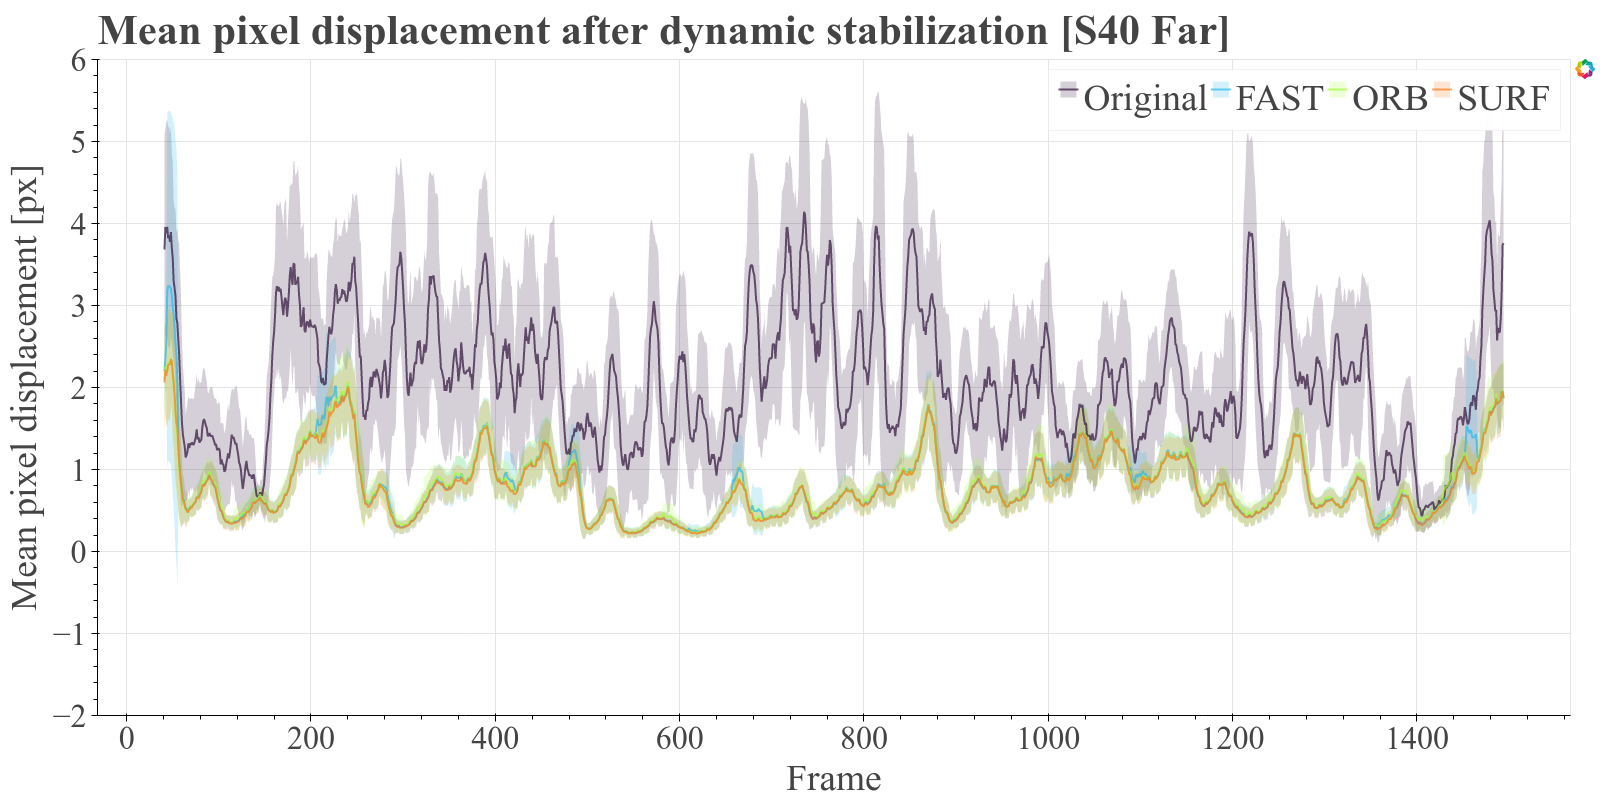
\includegraphics[width=0.475\linewidth]{diagrams/optical_flow/s40_n_far_image_raw.mp4.csv/compare_of_mean_pixel_displacement/window_size_12.html.png}    &  
      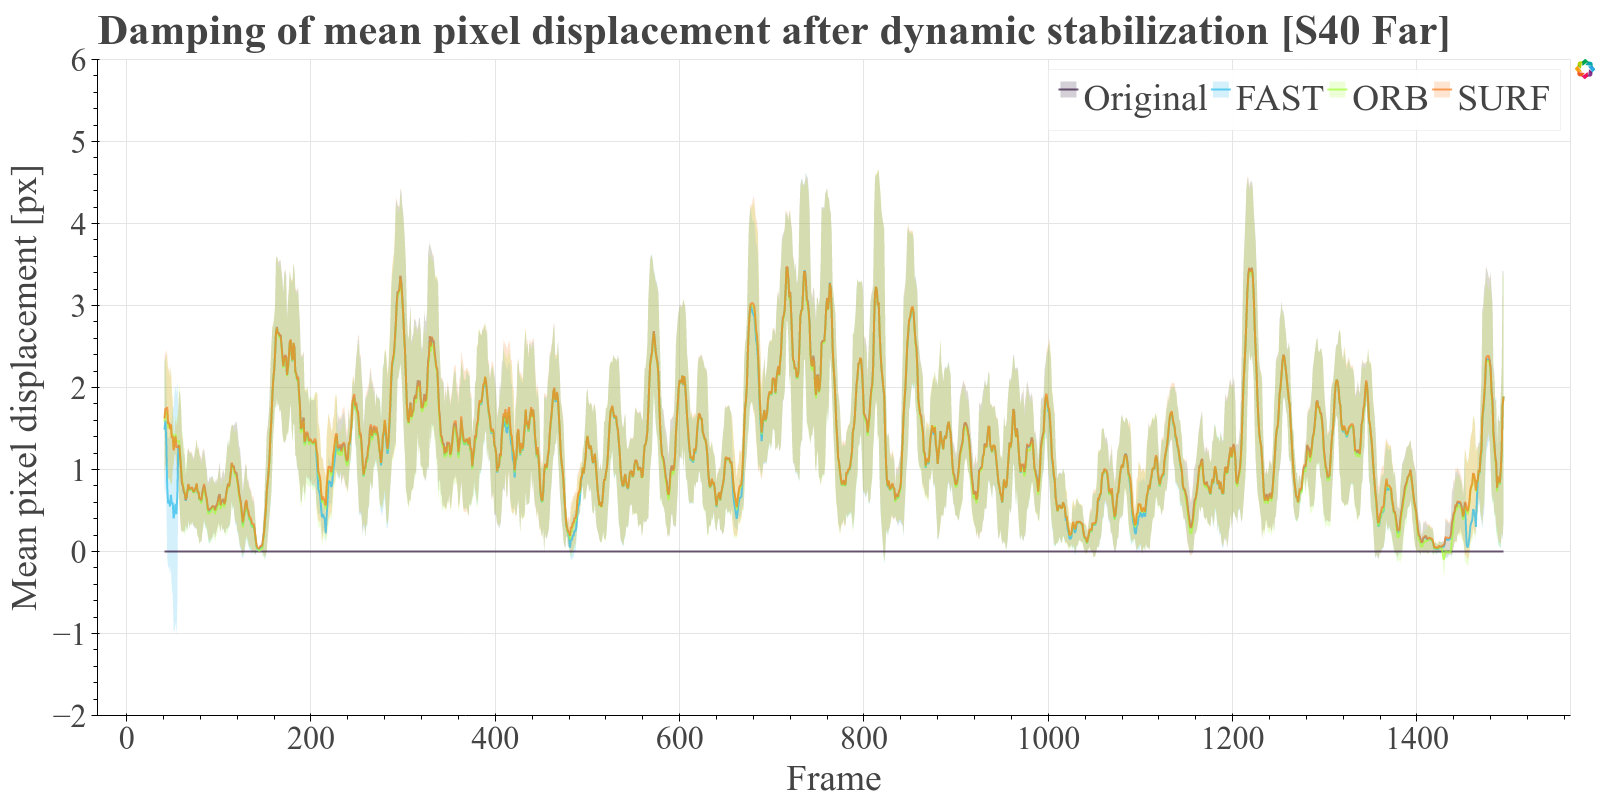
\includegraphics[width=0.475\linewidth]{diagrams/optical_flow/s40_n_far_image_raw.mp4.csv/deltas_of_mean_pixel_displacement/window_size_12.html.png}   \\ 

      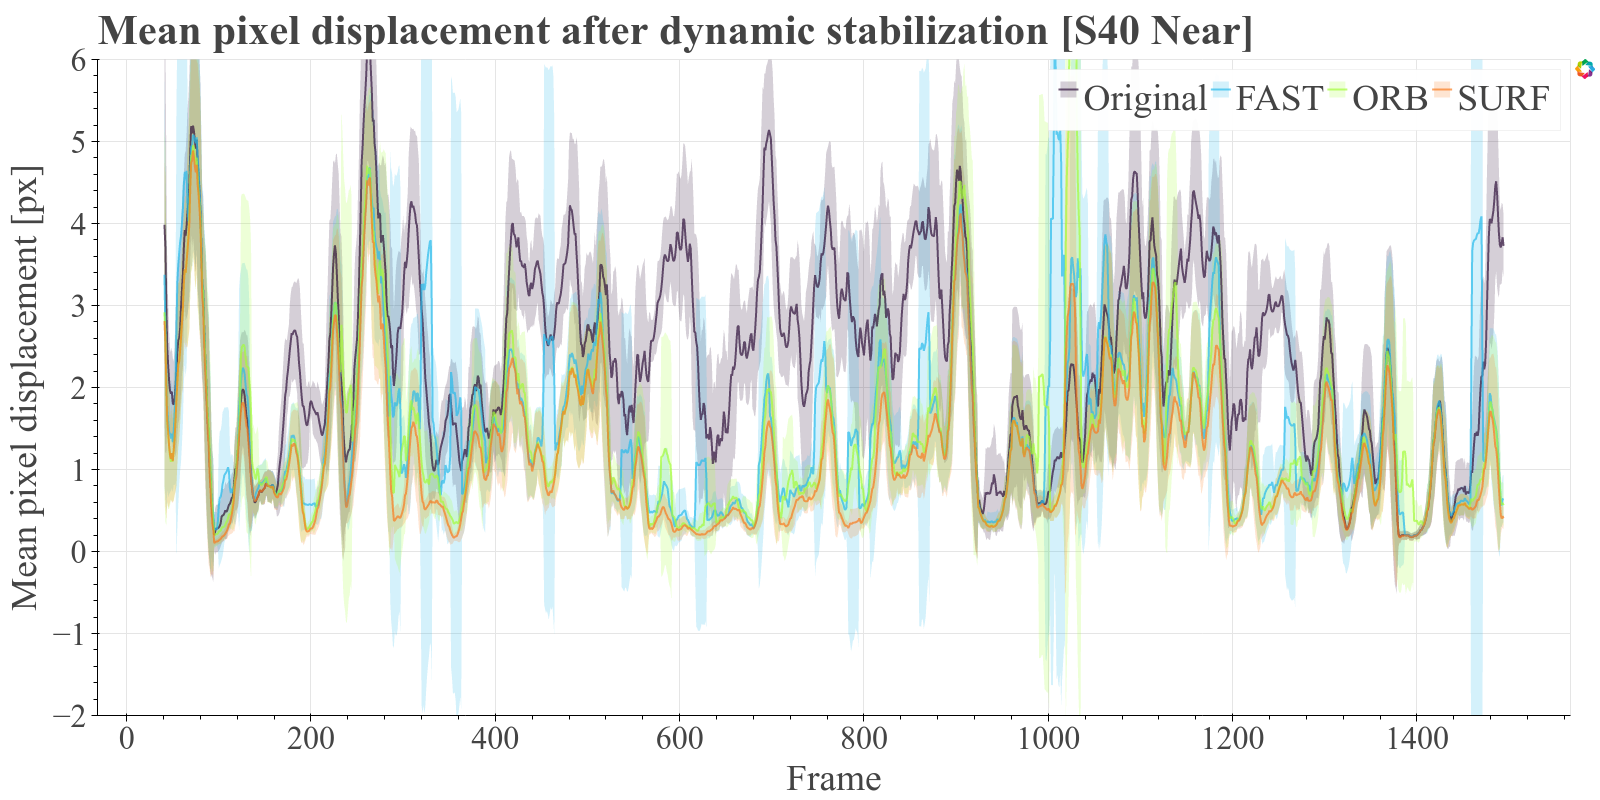
\includegraphics[width=0.475\linewidth]{diagrams/optical_flow/s40_n_near_image_raw.mp4.csv/compare_of_mean_pixel_displacement/window_size_12.html.png}    & 
      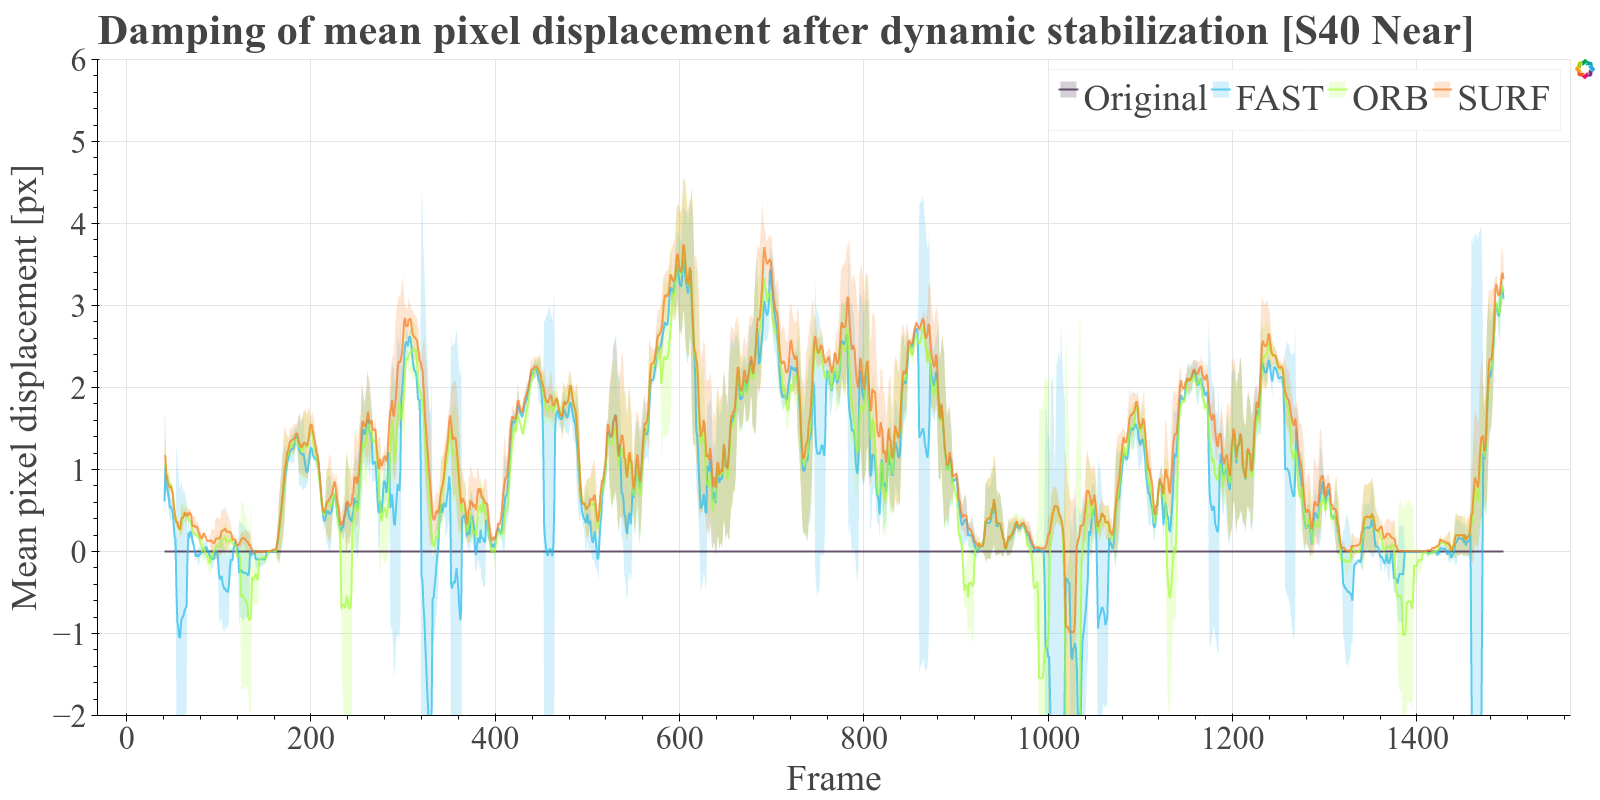
\includegraphics[width=0.475\linewidth]{diagrams/optical_flow/s40_n_near_image_raw.mp4.csv/deltas_of_mean_pixel_displacement/window_size_12.html.png}   \\ 

      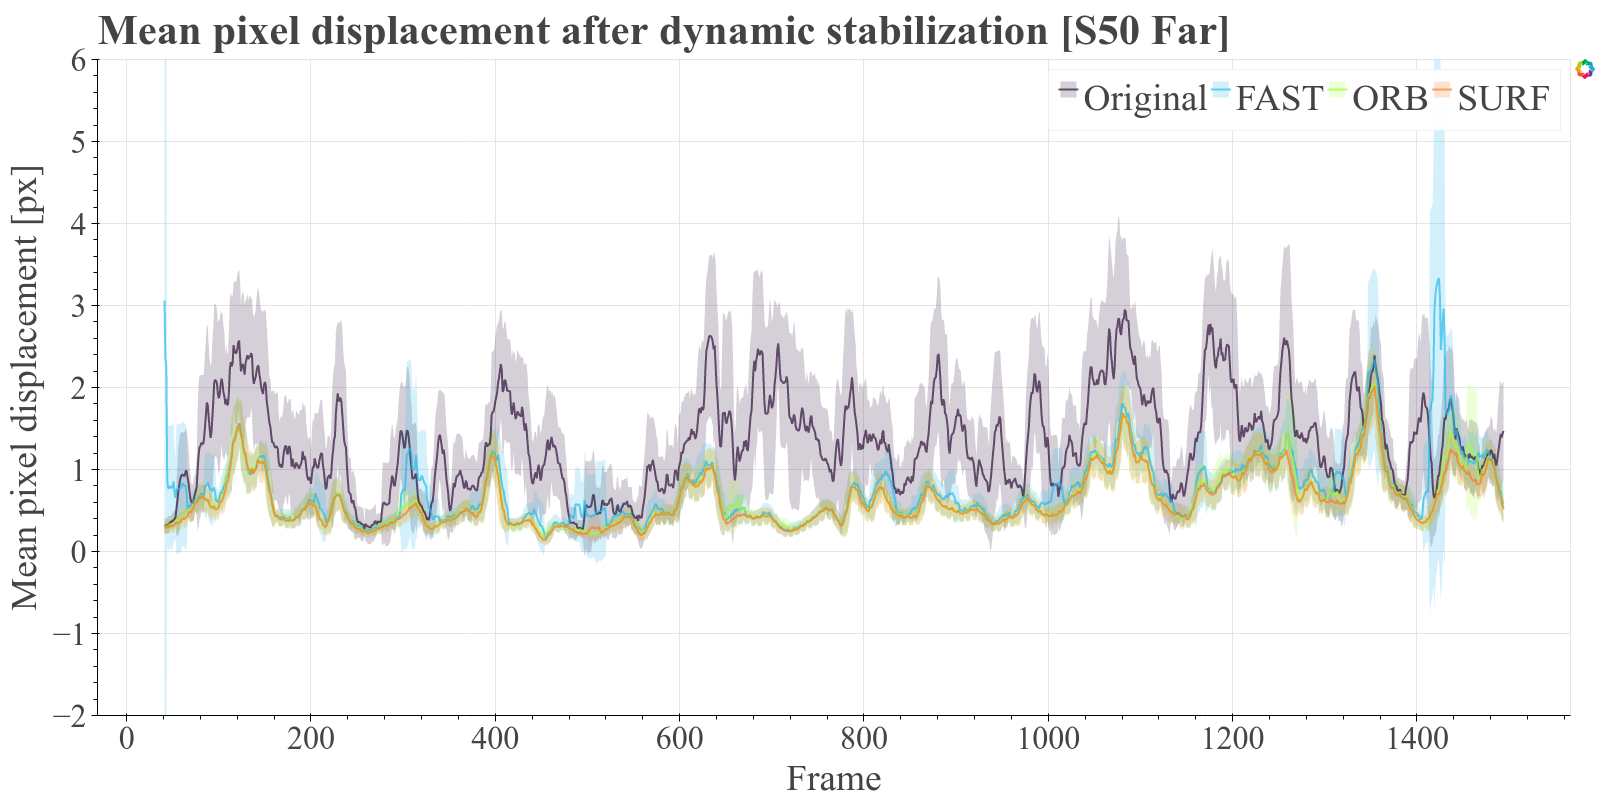
\includegraphics[width=0.475\linewidth]{diagrams/optical_flow/s50_s_far_image_raw.mp4.csv/compare_of_mean_pixel_displacement/window_size_12.html.png}    & 
      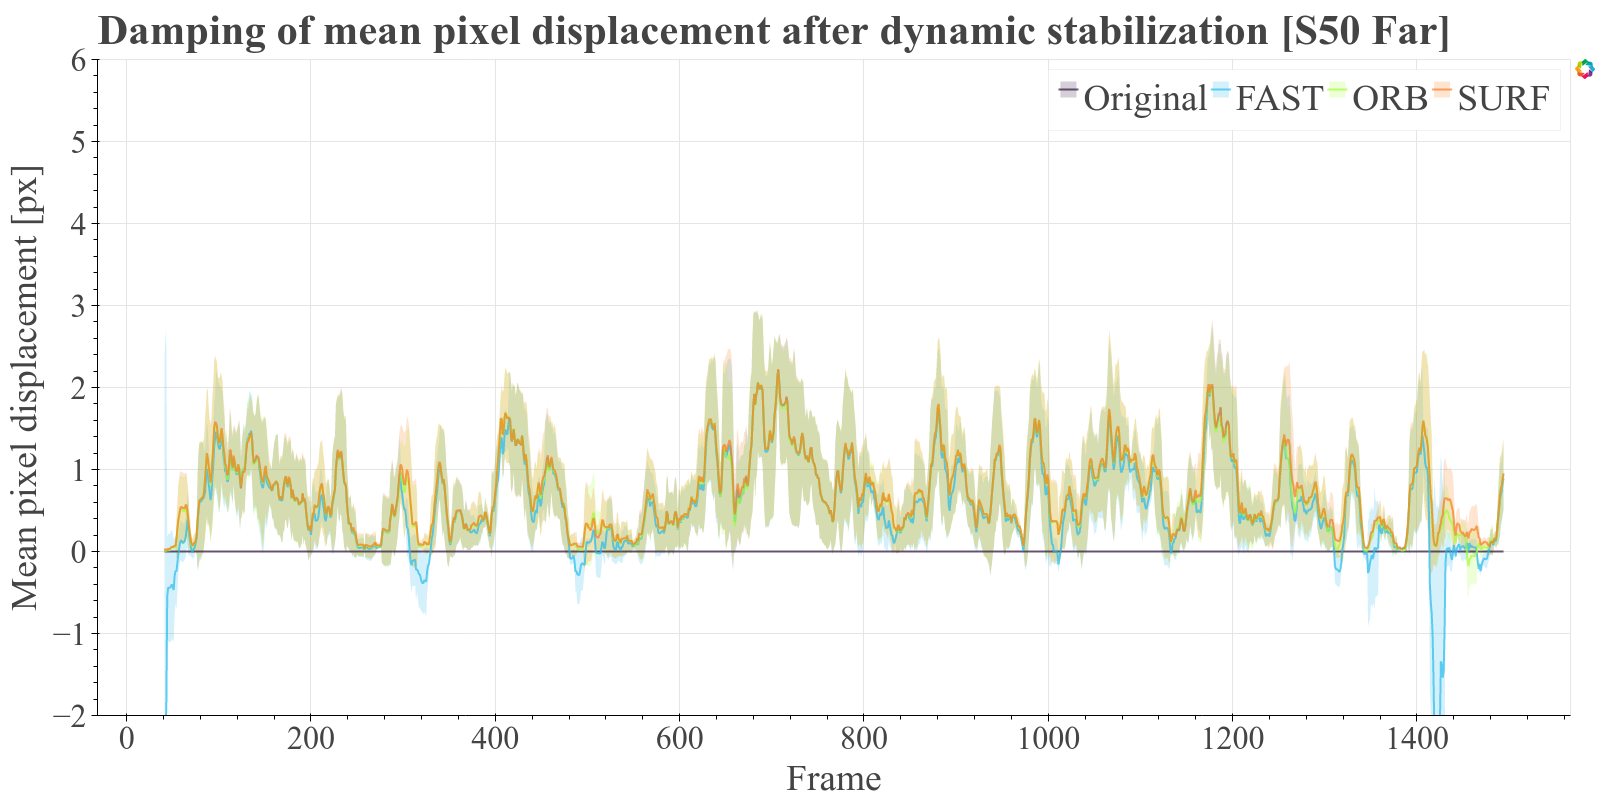
\includegraphics[width=0.475\linewidth]{diagrams/optical_flow/s50_s_far_image_raw.mp4.csv/deltas_of_mean_pixel_displacement/window_size_12.html.png}   \\ 

      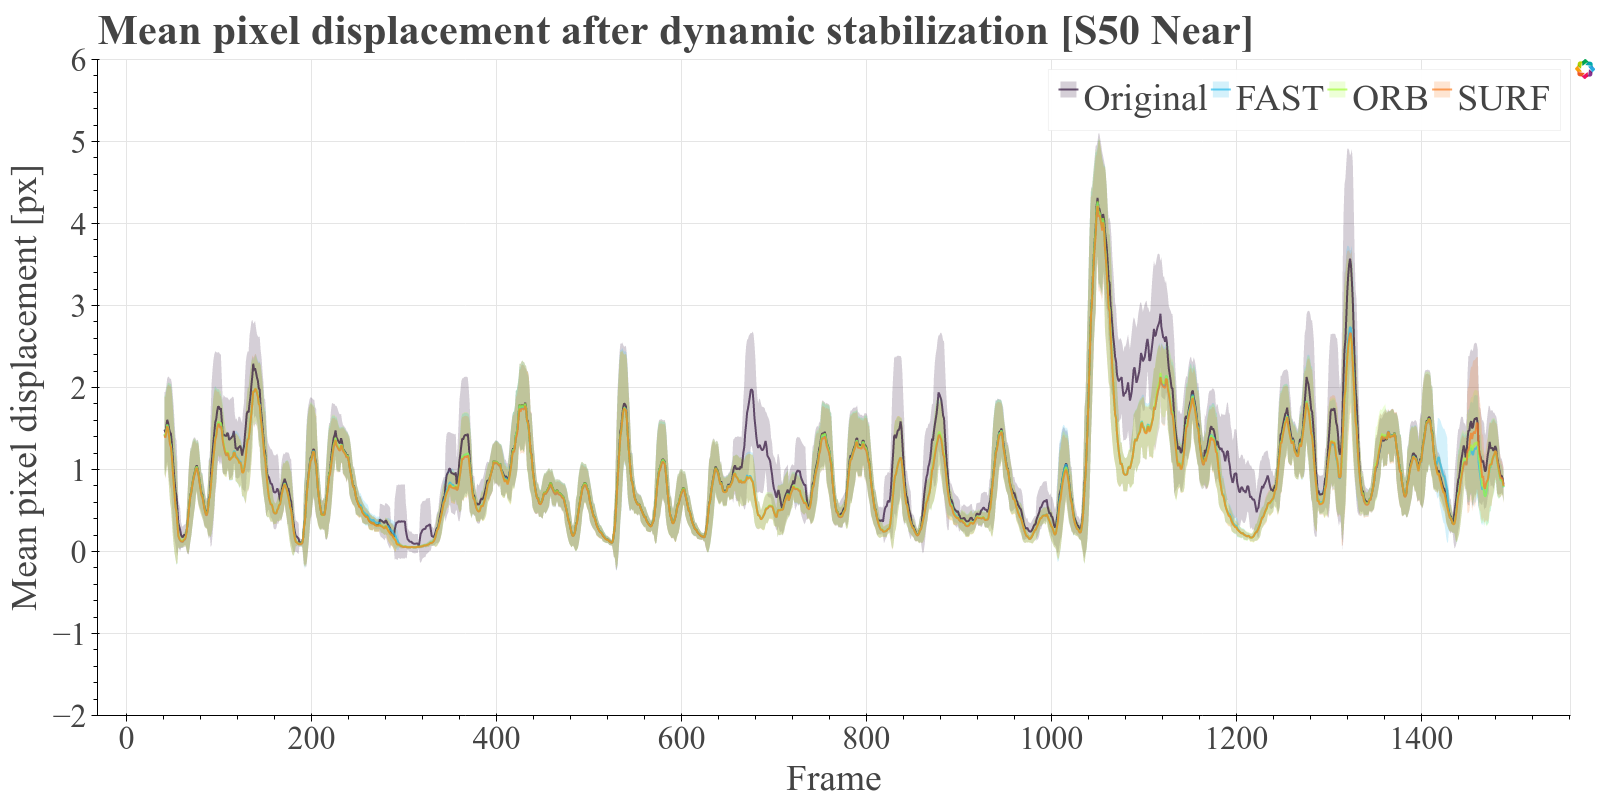
\includegraphics[width=0.475\linewidth]{diagrams/optical_flow/s50_s_near_image_raw.mp4.csv/compare_of_mean_pixel_displacement/window_size_12.html.png}    &   
      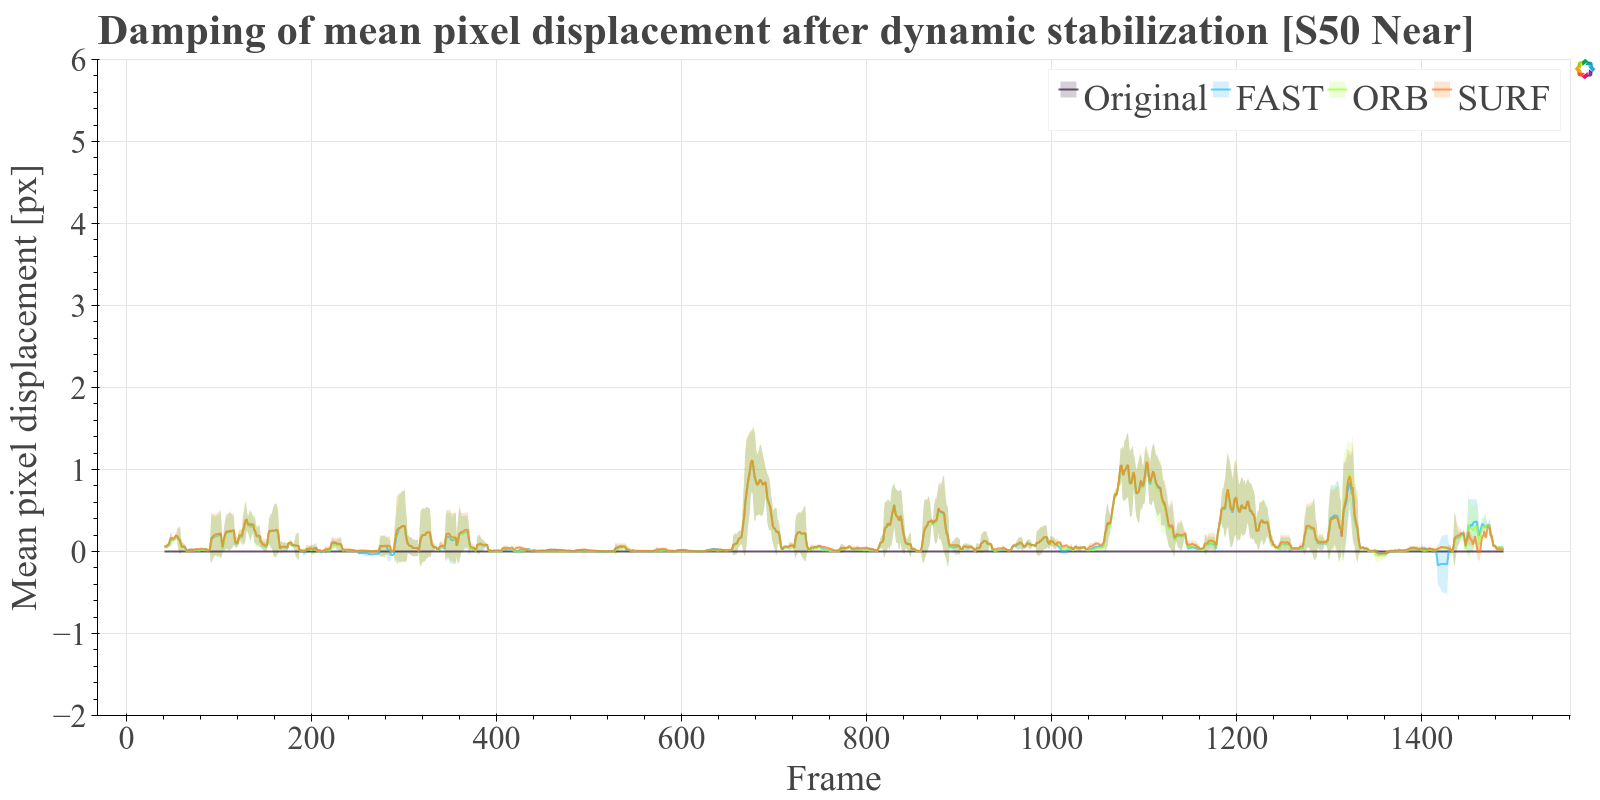
\includegraphics[width=0.475\linewidth]{diagrams/optical_flow/s50_s_near_image_raw.mp4.csv/deltas_of_mean_pixel_displacement/window_size_12.html.png}   \\ 
    \end{tabular}
    \caption{
        Left: 
        Comparison of the three implemented dynamic stabilizers and the original not stabilized video feed using Optical Flow as metric (lower is better).
        The stabilizers are based on the 
        FAST \cite{Ghahremani_2021,opencv_library} feature detector with FREAK \cite{alahi6247715,opencv_library} feature descriptors,
        SURF \cite{bay10.1007/11744023_32,opencv_library} feature detector and
        ORB \cite{rublee6126544, opencv_library} feature detector.
        The graphs display the mean pixel shift at each frame. 
        Right: 
        The damping capabilities of the same three stabilizers (higher is better). 
        The graphs approximate the removed jitter in the mean pixel shift between the original video and the stabilizer at each frame.\\
        For visualization the values are filtered using the rolling mean over 12 frames. 
        The light areas display the standard deviation within the window.
    }
    \label{fig:dynamic_stabilization_appendix}
    \end{figure*}

    



\begin{figure*}[!ht]
  \centering
  \begin{tabular}{cc}
    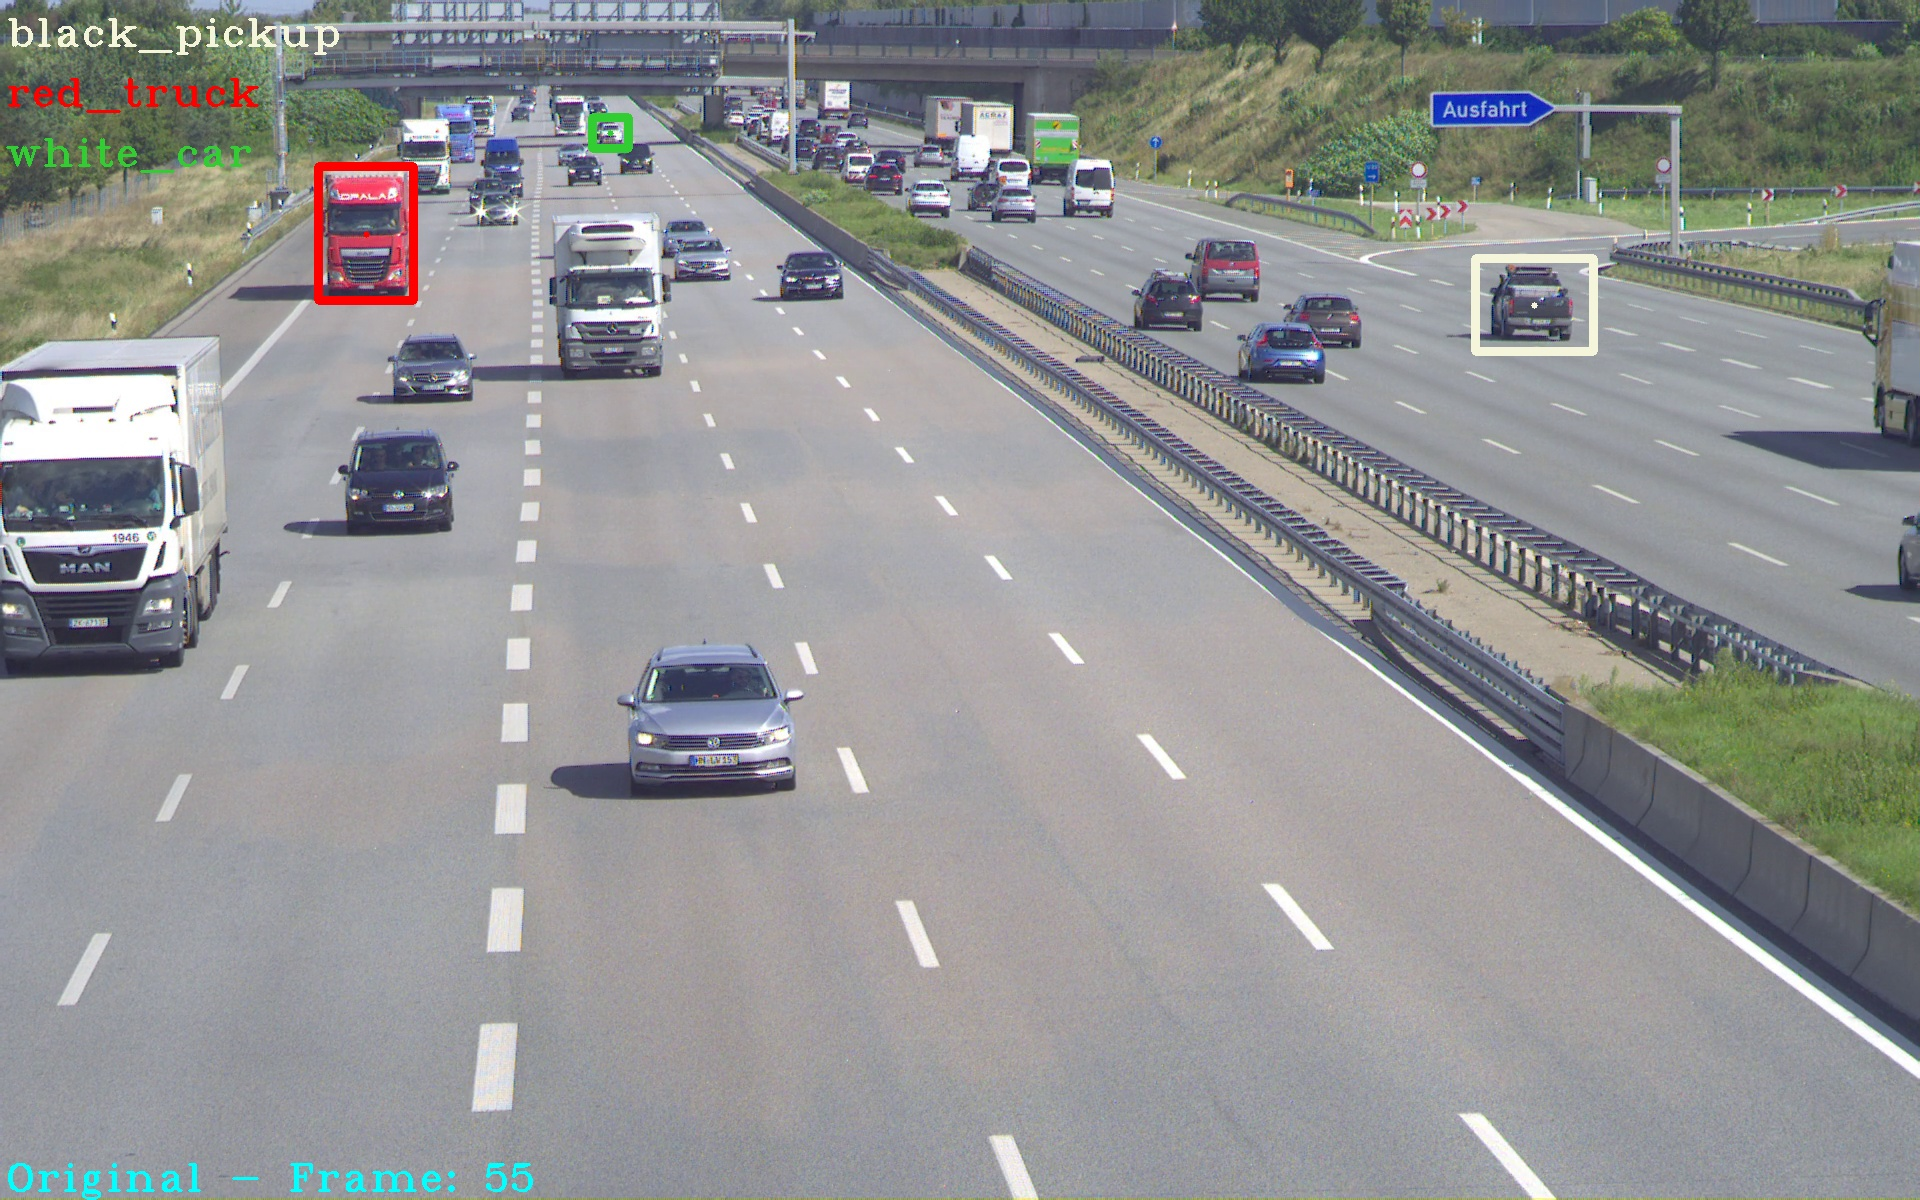
\includegraphics[width=0.45\linewidth]{diagrams/object_tracking/s40_n_far/frame.png}    &  
    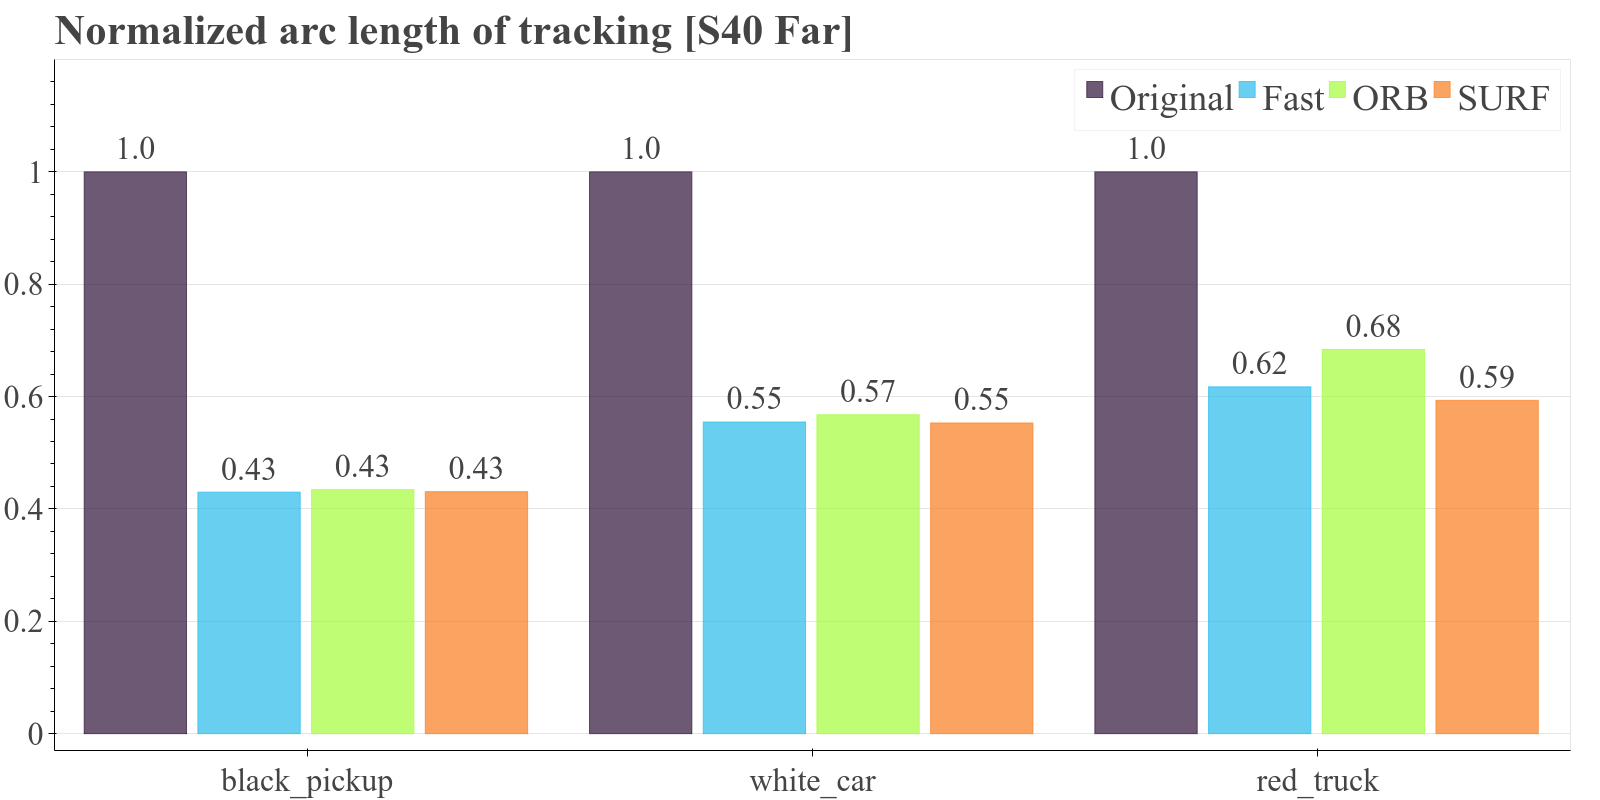
\includegraphics[width=0.475\linewidth]{diagrams/object_tracking/s40_n_far/arcs.png}    \\

    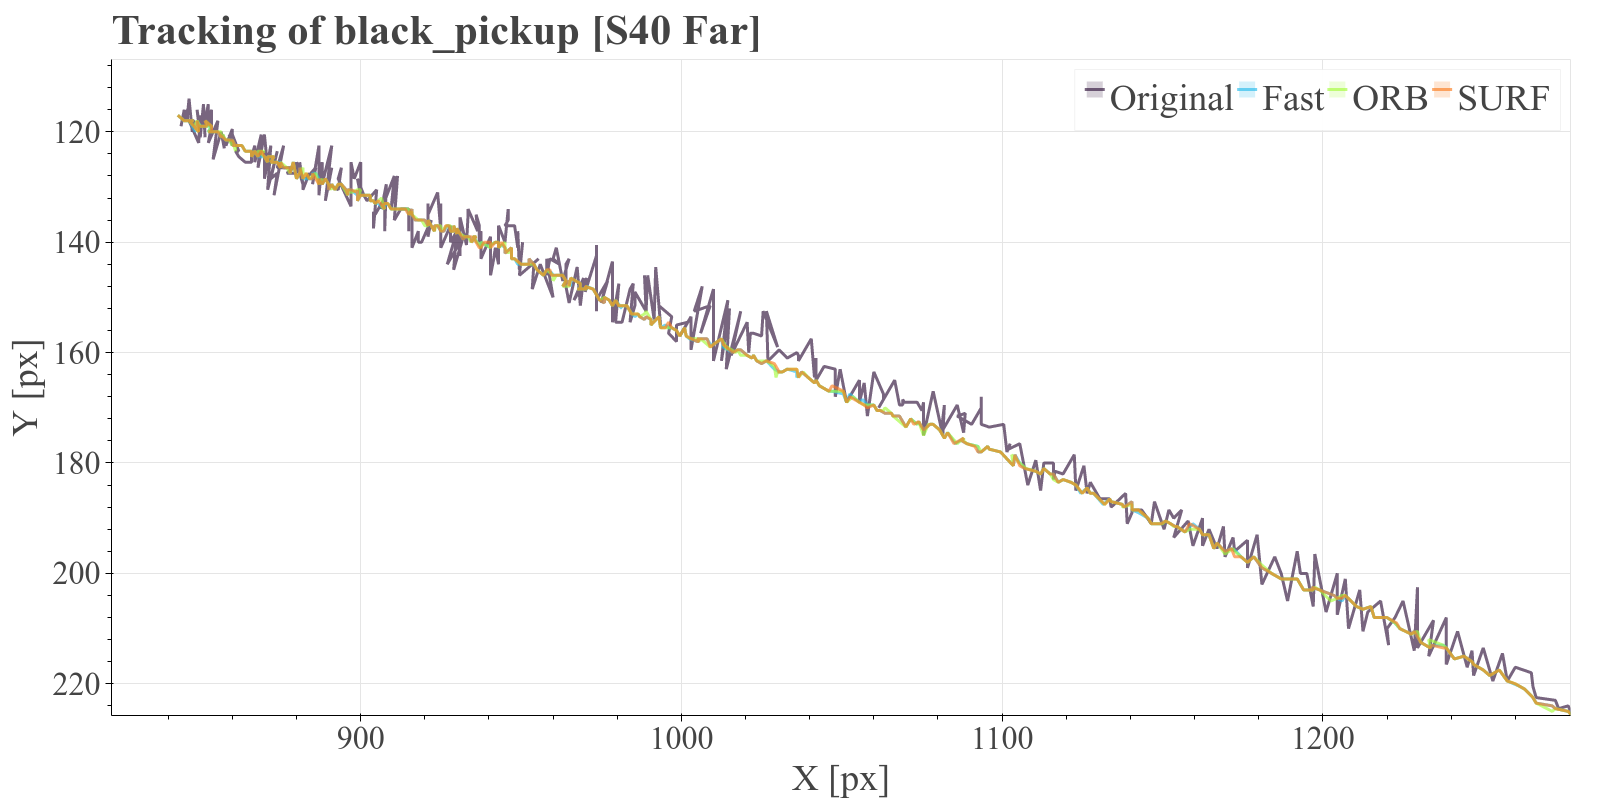
\includegraphics[width=0.475\linewidth]{diagrams/object_tracking/s40_n_far/black_pickup.png}    &  
    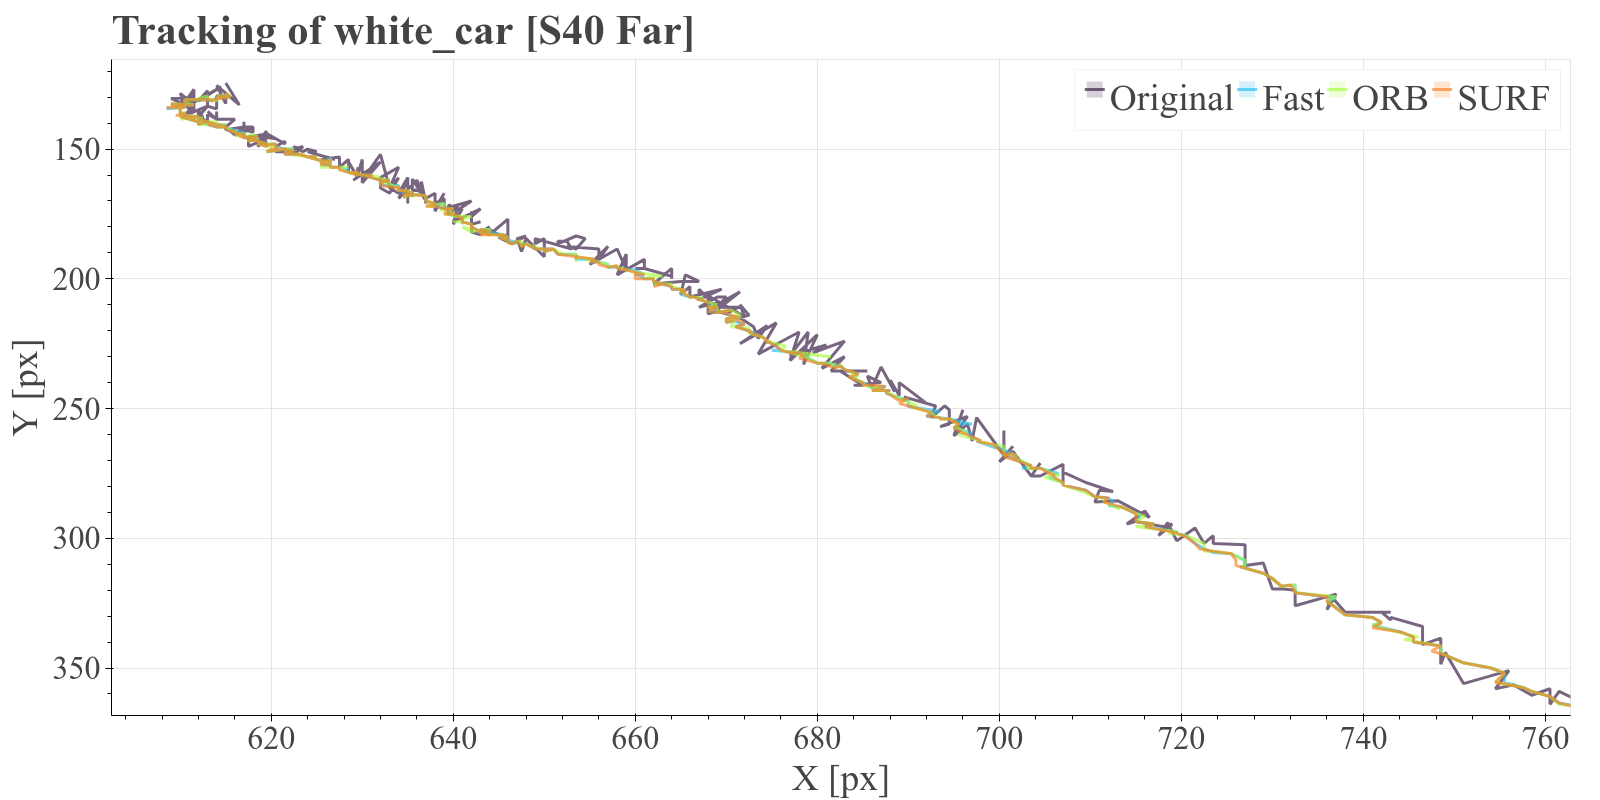
\includegraphics[width=0.475\linewidth]{diagrams/object_tracking/s40_n_far/white_car.png}    \\  
    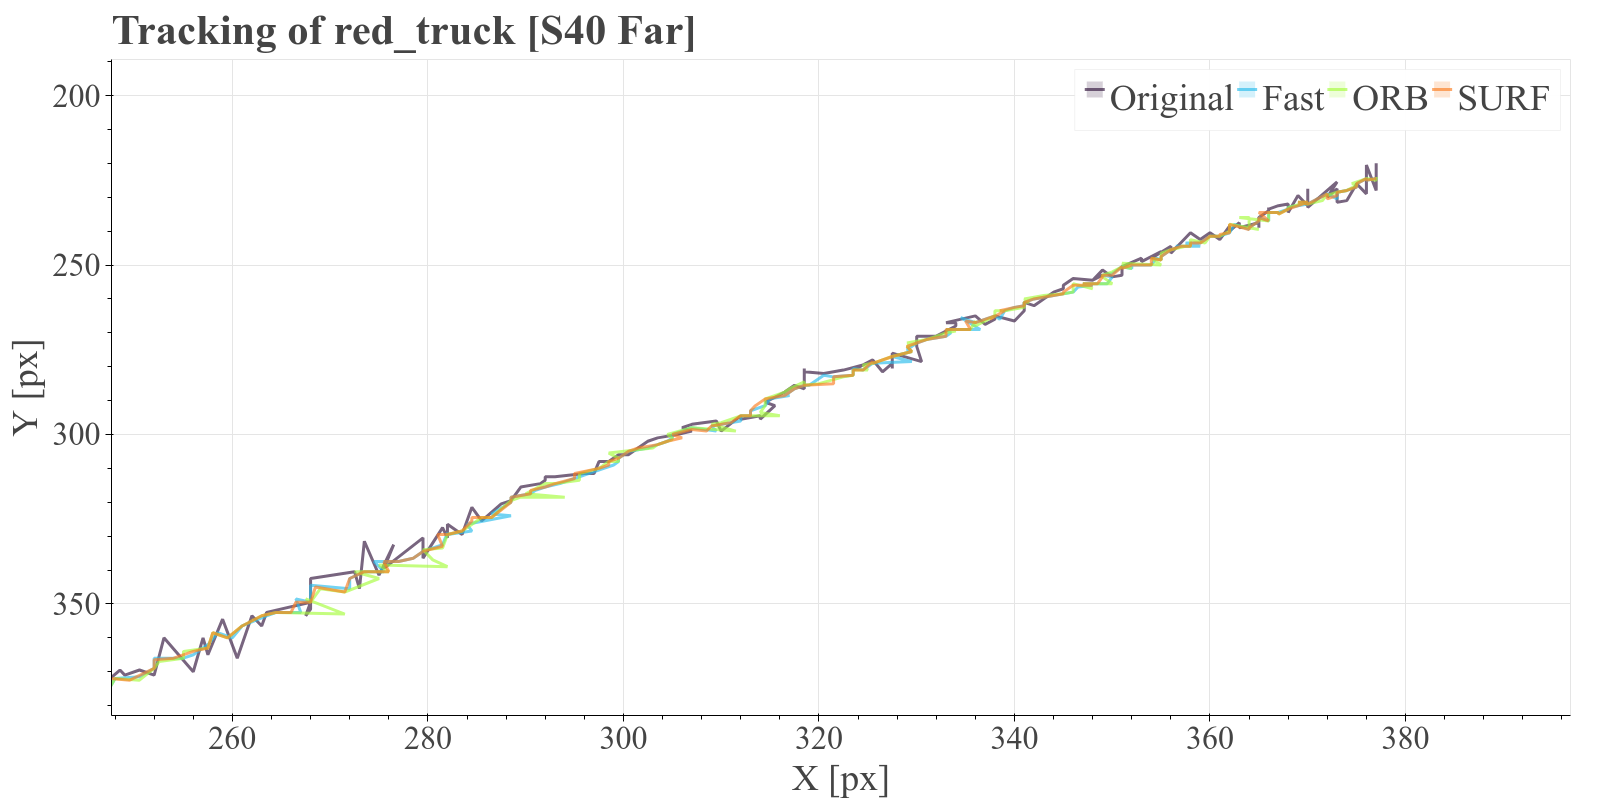
\includegraphics[width=0.475\linewidth]{diagrams/object_tracking/s40_n_far/red_truck.png}   
  \end{tabular}
  \caption{Left: 
  The exemplary vehicles tracked through the video sequence of the camera \camsn{4}. 
  Right:
  The corresponding normalized arc lengths of the pixel path. 
  The length is normalized by the original arc length, hence the 1.0 factor for the original video. 
  As the jitter is removed, the pixels movement is lowered significantly as it does only move with the vehicle, not the camera.
  This can be seen with around half of the path length remaining after stabilization for all stabilizers.
  }
  \label{fig:object_tracking_appendix_s40_n_far}
\end{figure*}



\begin{figure*}[!ht]
  \centering
  \begin{tabular}{cc}
    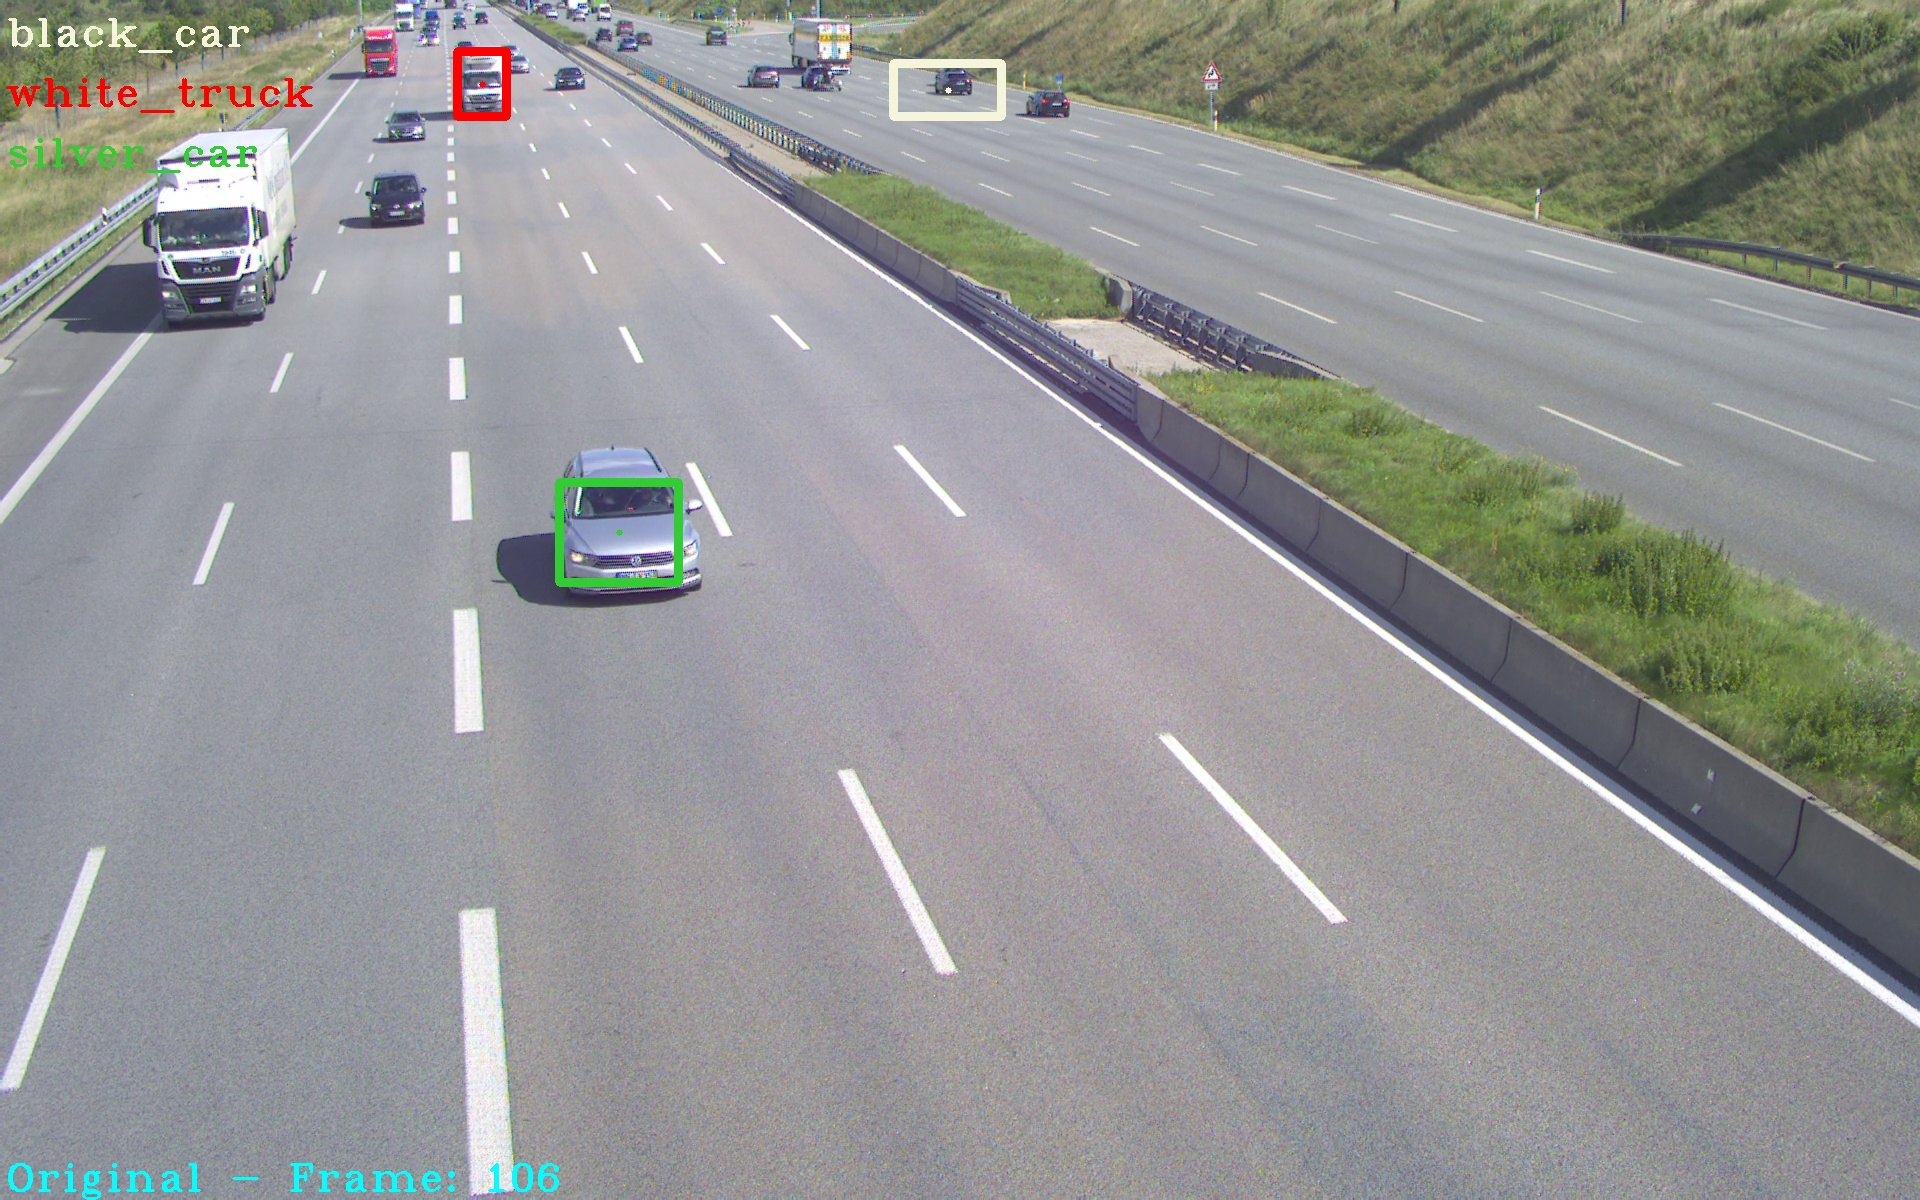
\includegraphics[width=0.45\linewidth]{diagrams/object_tracking/s40_n_near/frame.png}    &  
    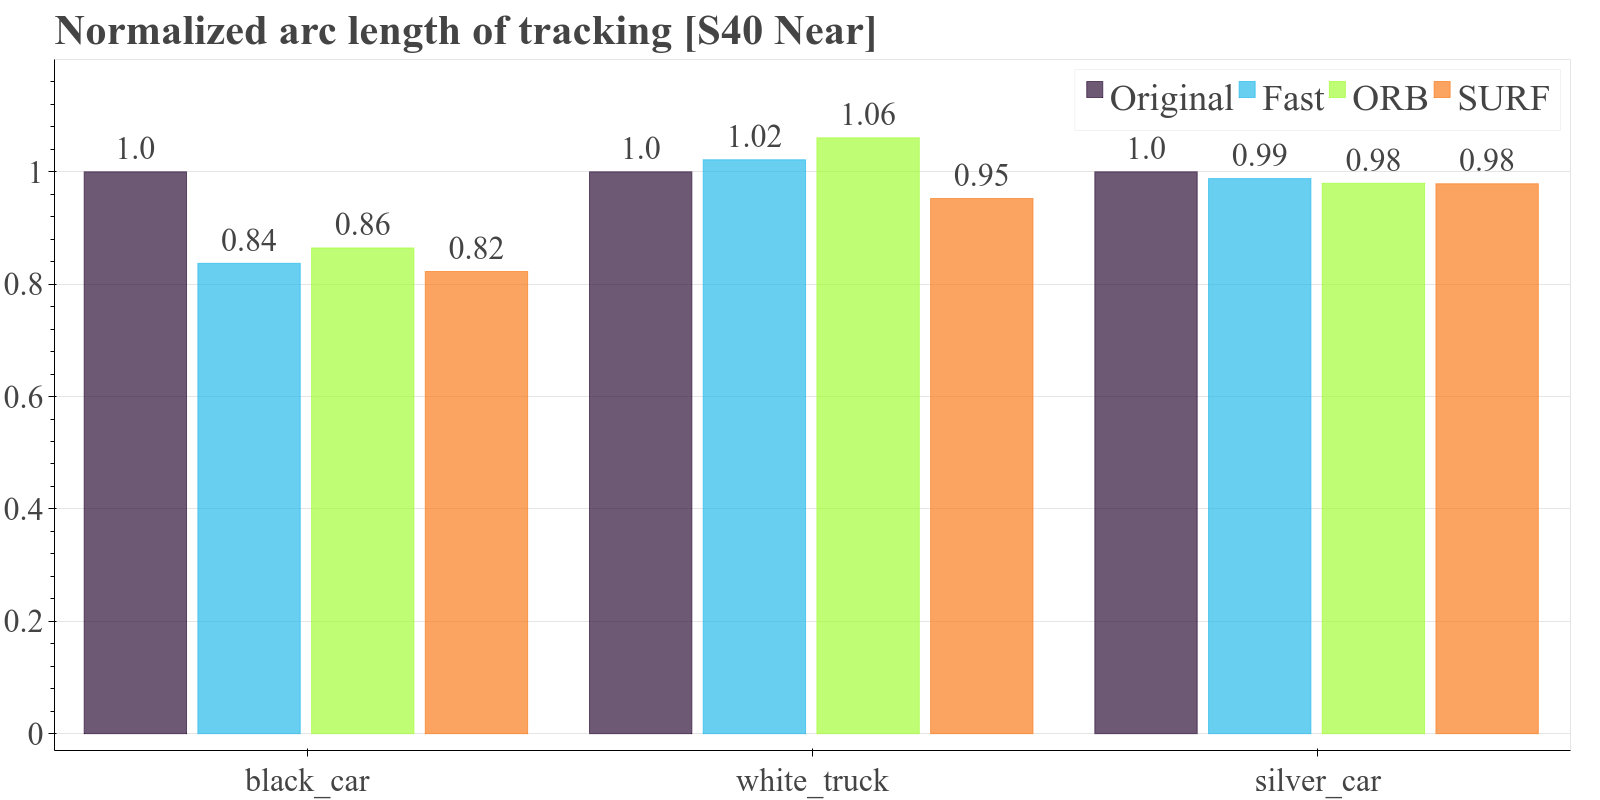
\includegraphics[width=0.475\linewidth]{diagrams/object_tracking/s40_n_near/arcs.png}    \\

    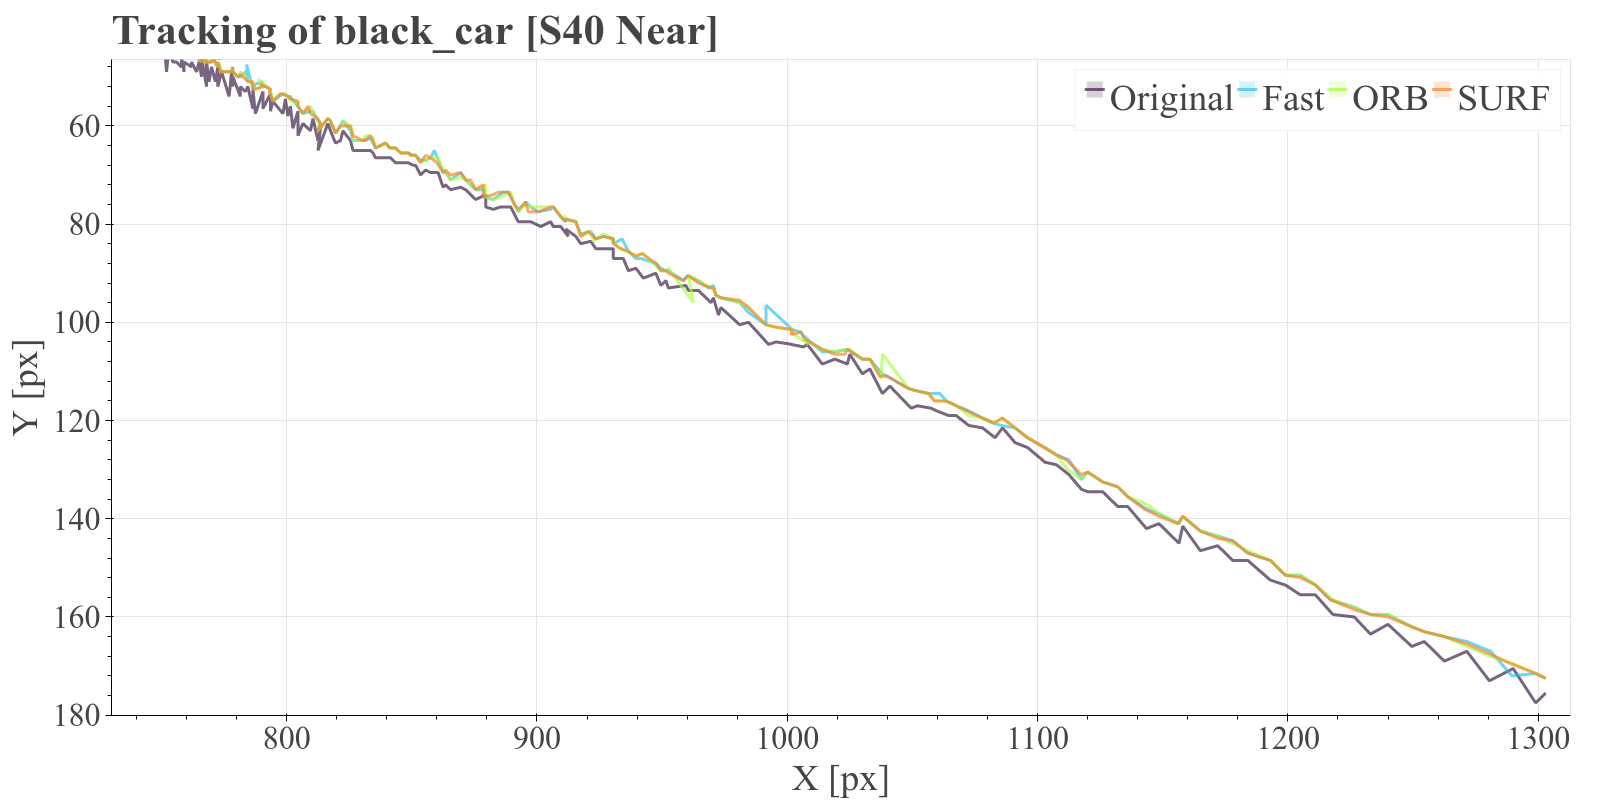
\includegraphics[width=0.475\linewidth]{diagrams/object_tracking/s40_n_near/black_car.png}    &  
    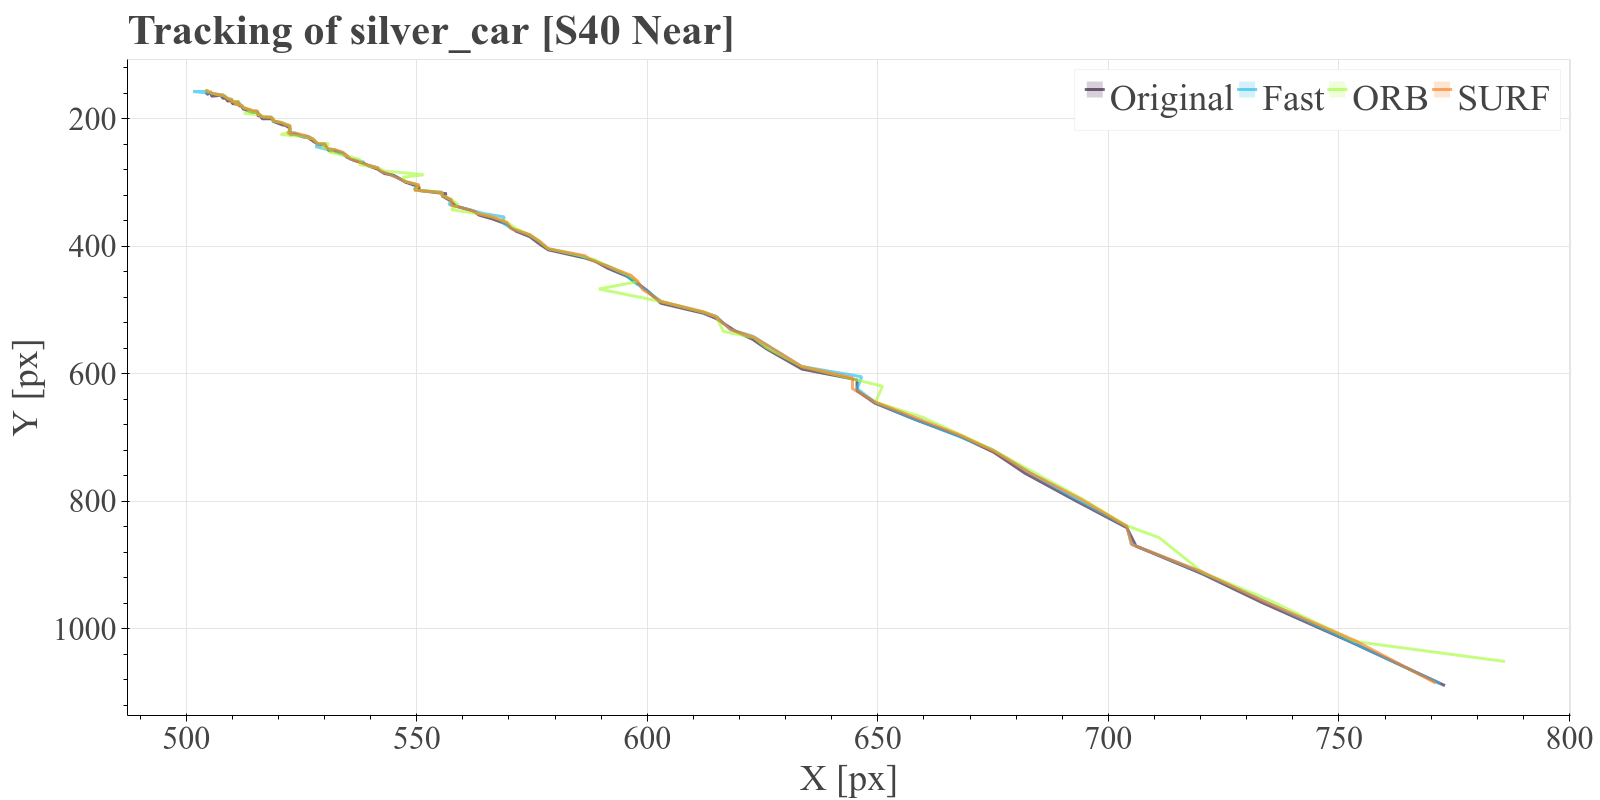
\includegraphics[width=0.475\linewidth]{diagrams/object_tracking/s40_n_near/silver_car.png}    \\  
    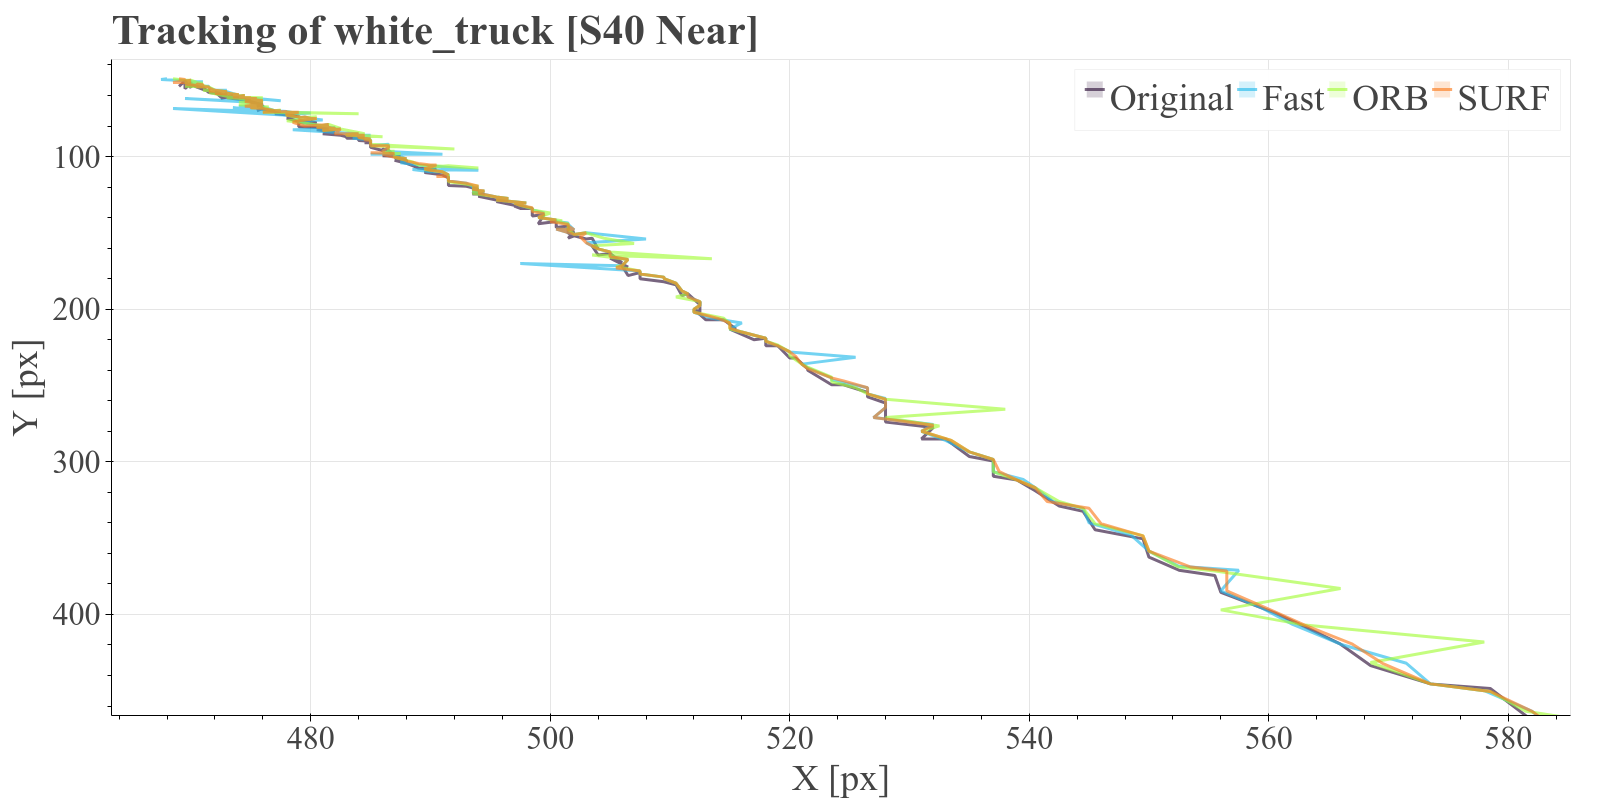
\includegraphics[width=0.475\linewidth]{diagrams/object_tracking/s40_n_near/white_truck.png}   
  \end{tabular}
  \caption{Left: 
  The exemplary vehicles tracked through the video sequence of the camera \camsn{4}. 
  Right:
  The corresponding normalized arc lengths of the pixel path. 
  The length is normalized by the original arc length, hence the 1.0 factor for the original video. 
  As the jitter is removed, the pixels movement is lowered significantly as it does only move with the vehicle, not the camera.
  This can be seen with around half of the path length remaining after stabilization for all stabilizers.
  }
  \label{fig:object_tracking_appendix_s40_n_near}
\end{figure*}



\begin{figure*}[!ht]
  \centering
  \begin{tabular}{cc}
    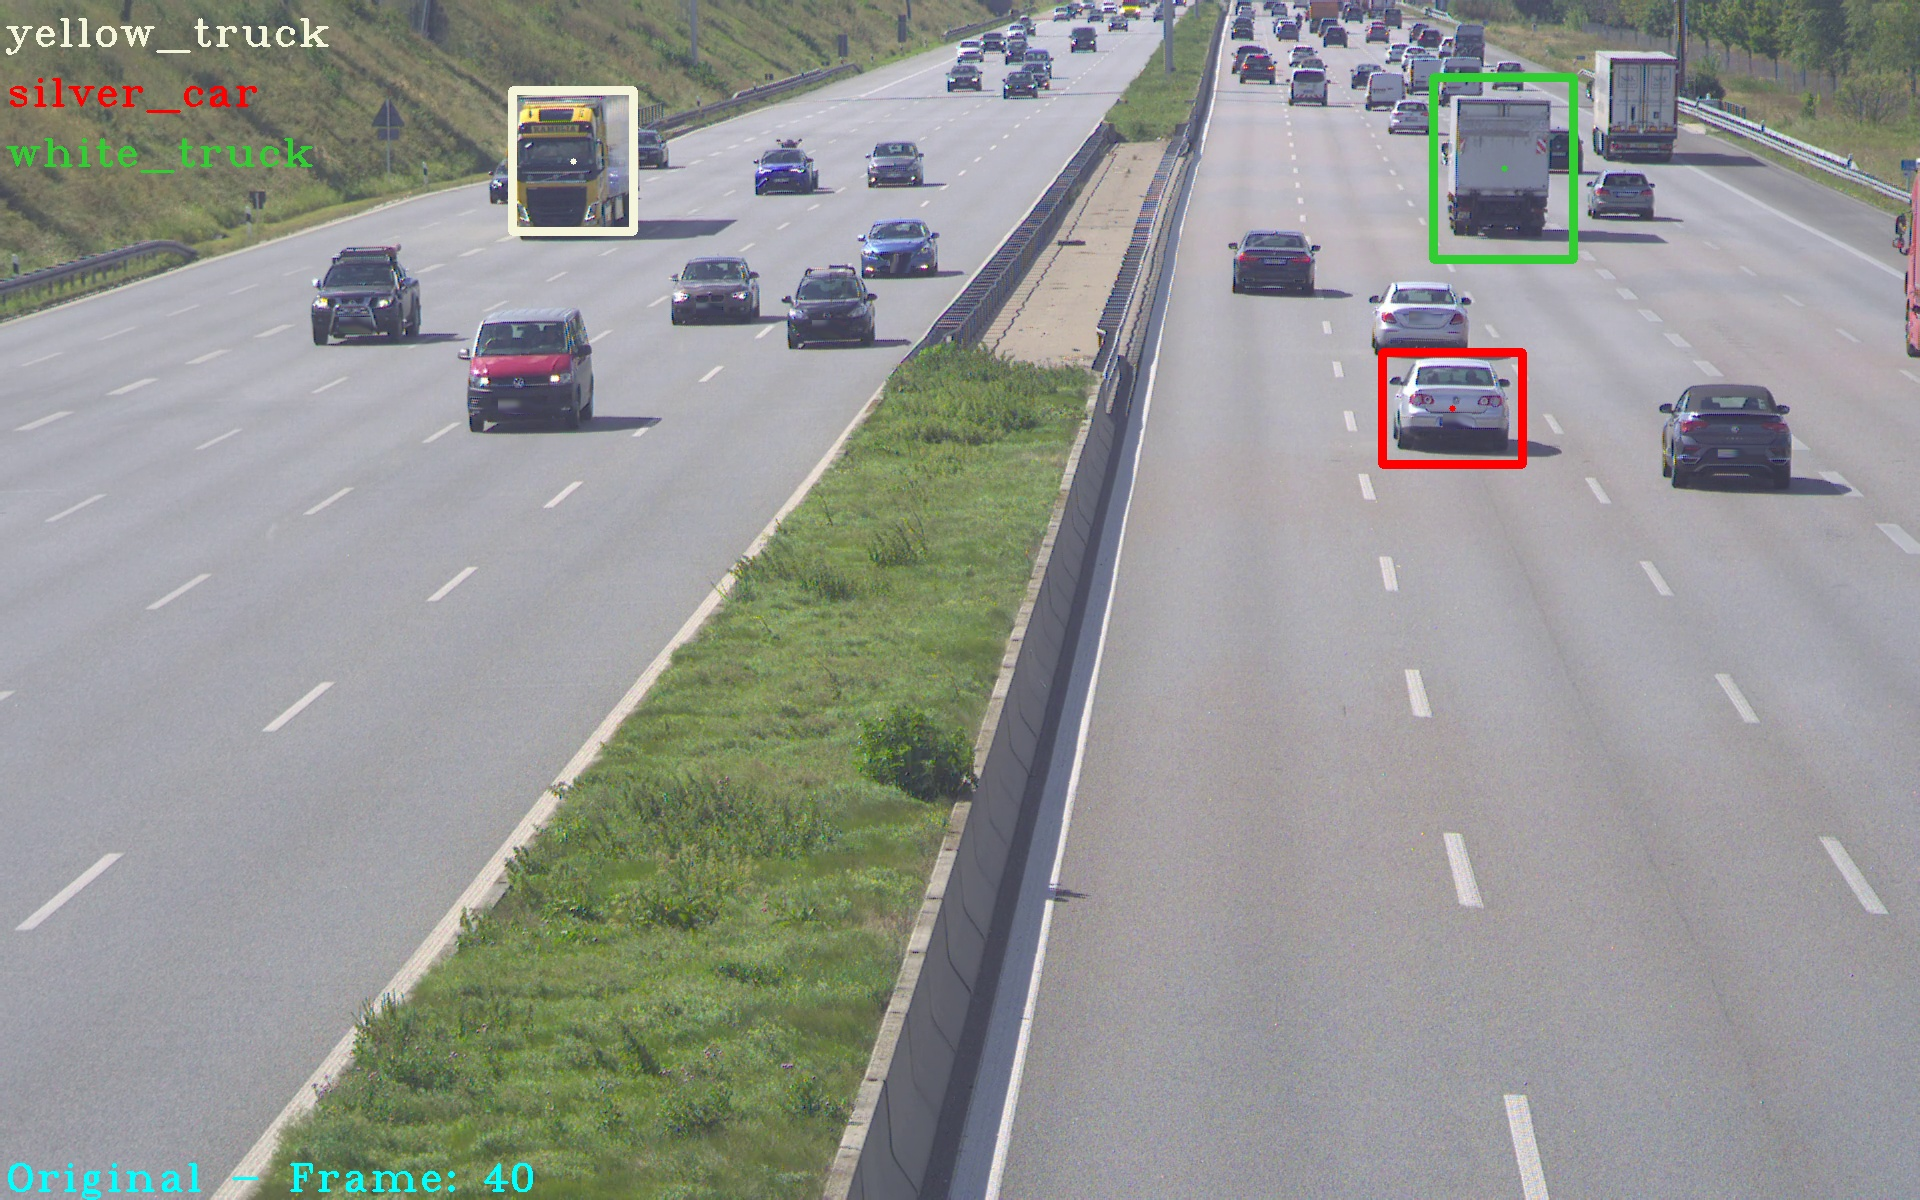
\includegraphics[width=0.45\linewidth]{diagrams/object_tracking/s50_s_far/frame.png}    &  
    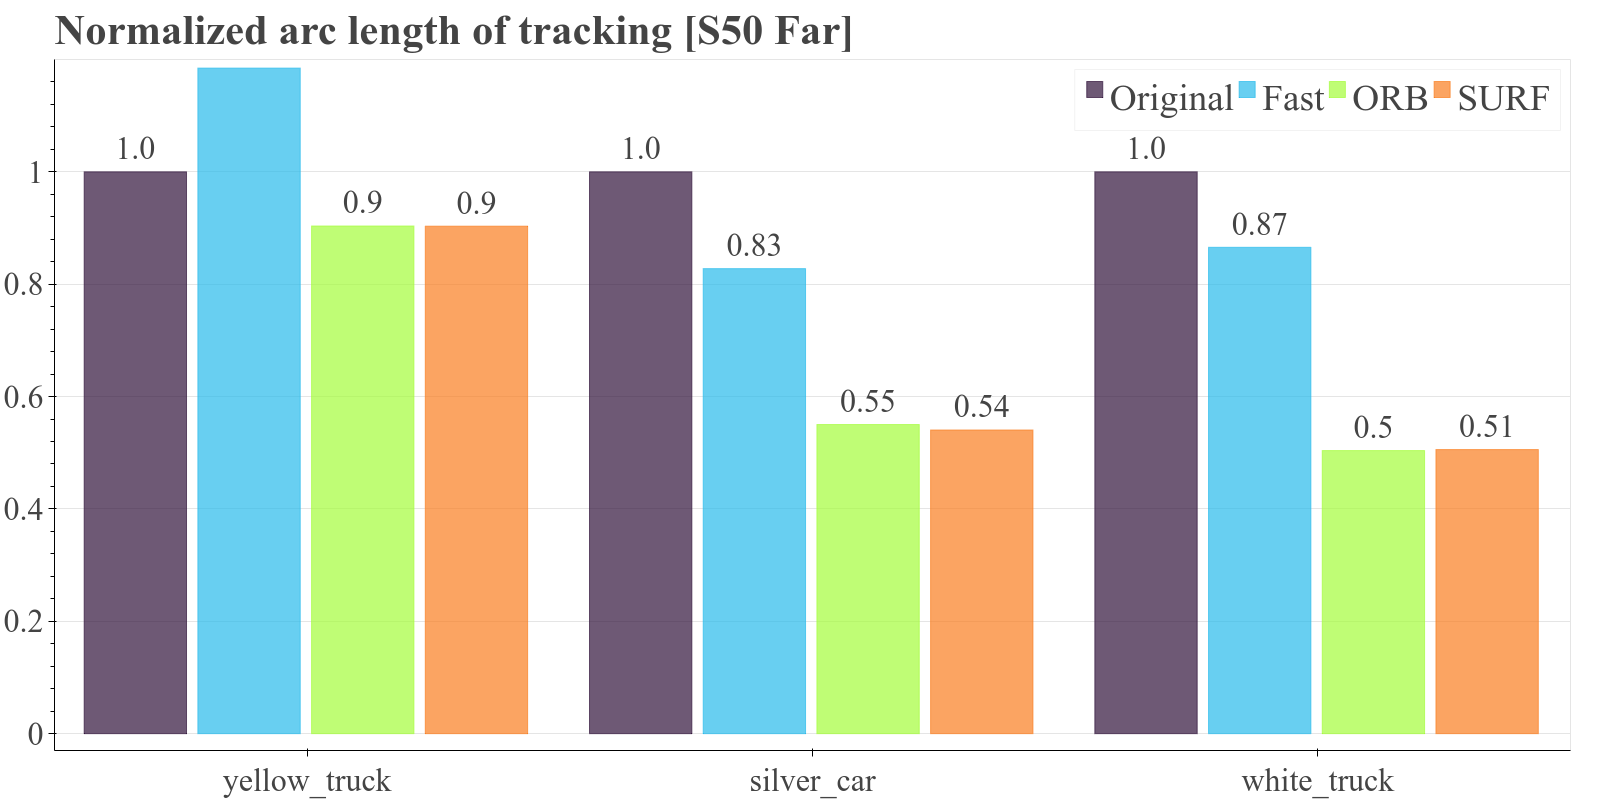
\includegraphics[width=0.475\linewidth]{diagrams/object_tracking/s50_s_far/arcs.png}    \\

    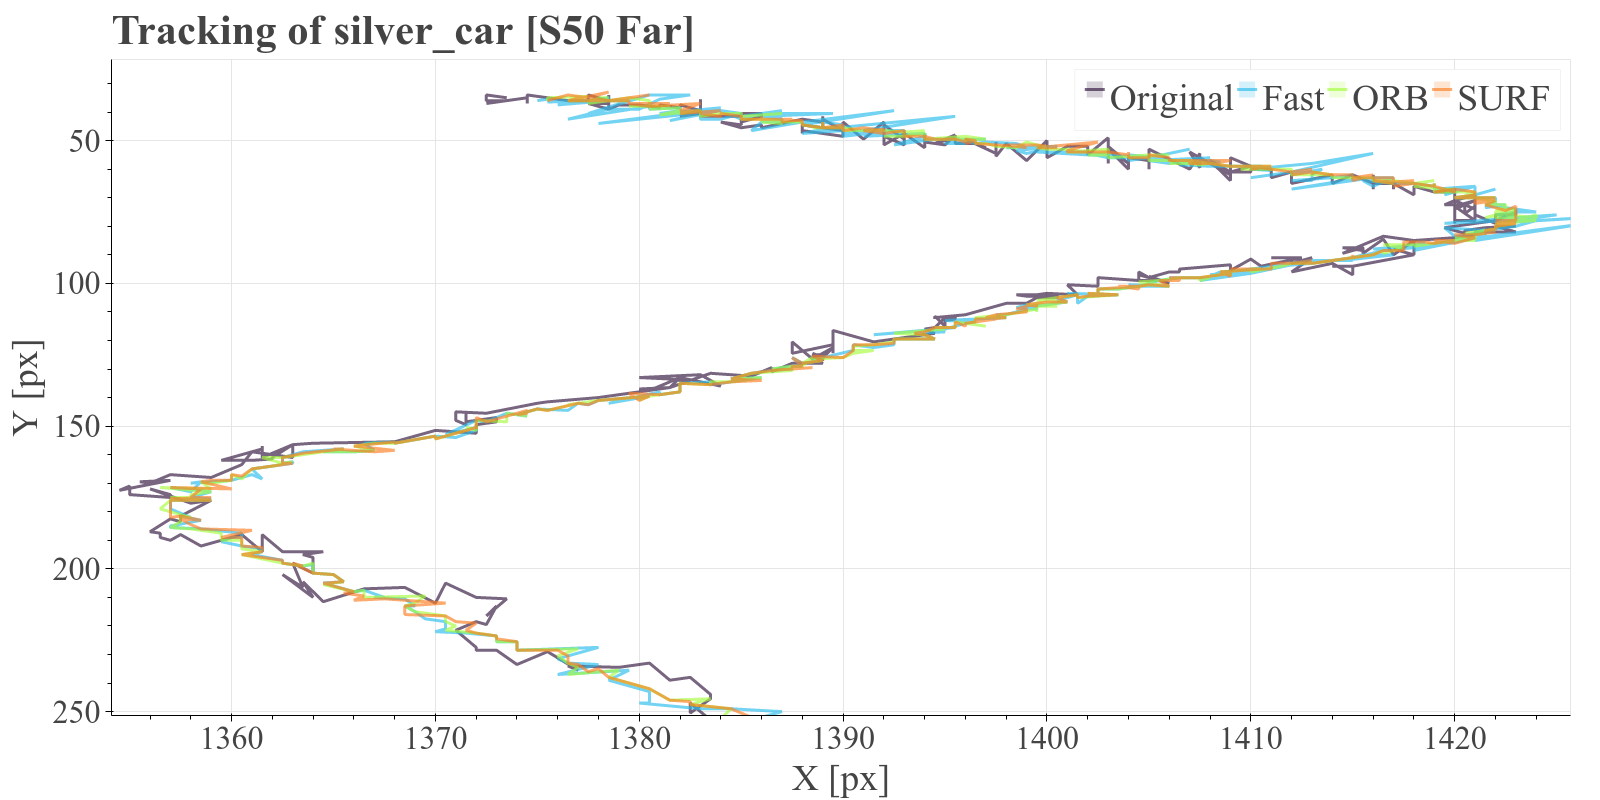
\includegraphics[width=0.475\linewidth]{diagrams/object_tracking/s50_s_far/silver_car.png}    &  
    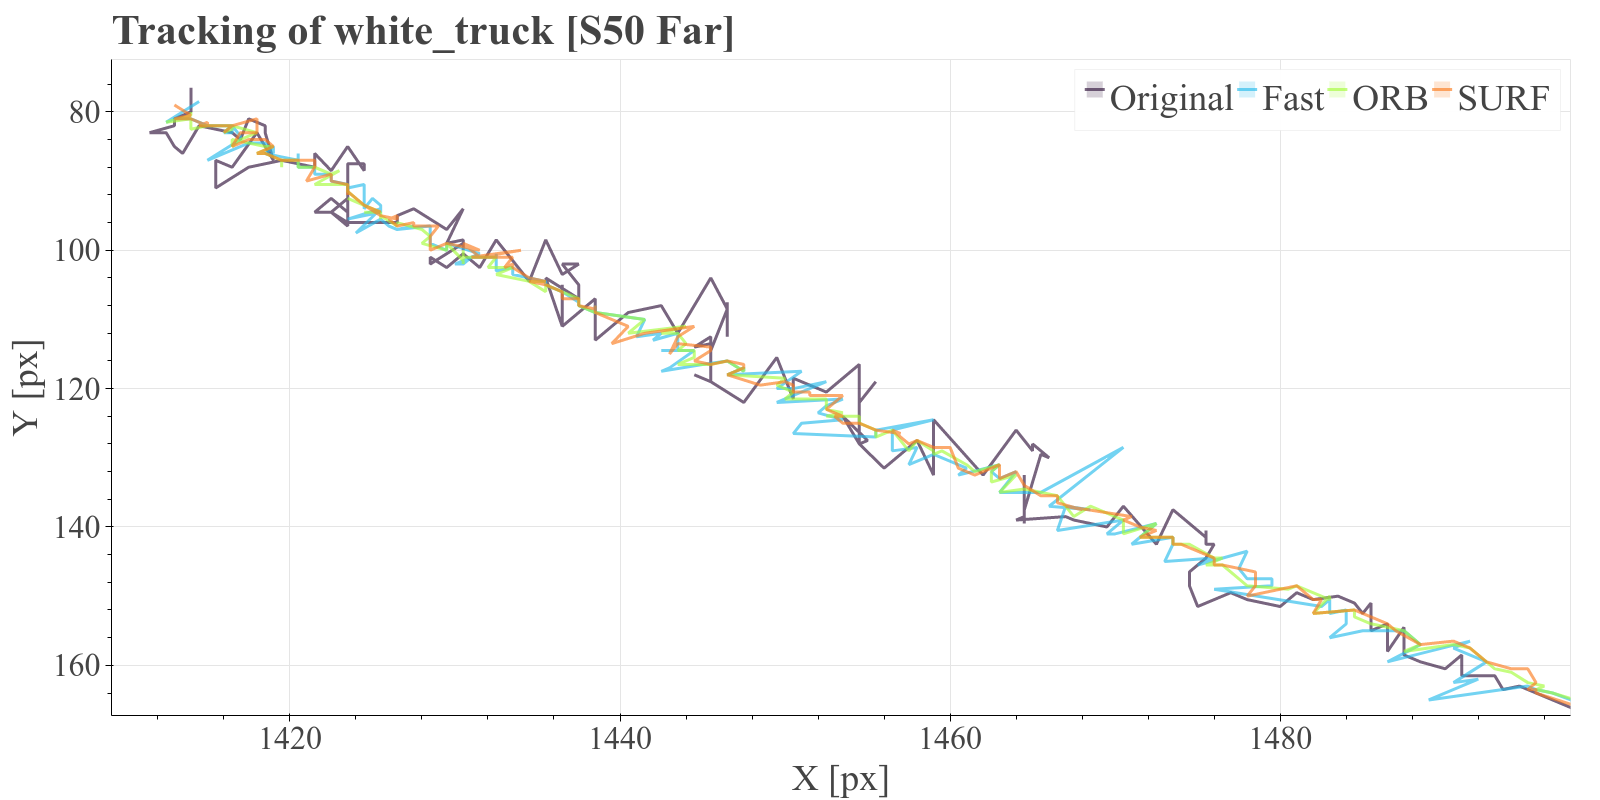
\includegraphics[width=0.475\linewidth]{diagrams/object_tracking/s50_s_far/white_truck.png}    \\  
    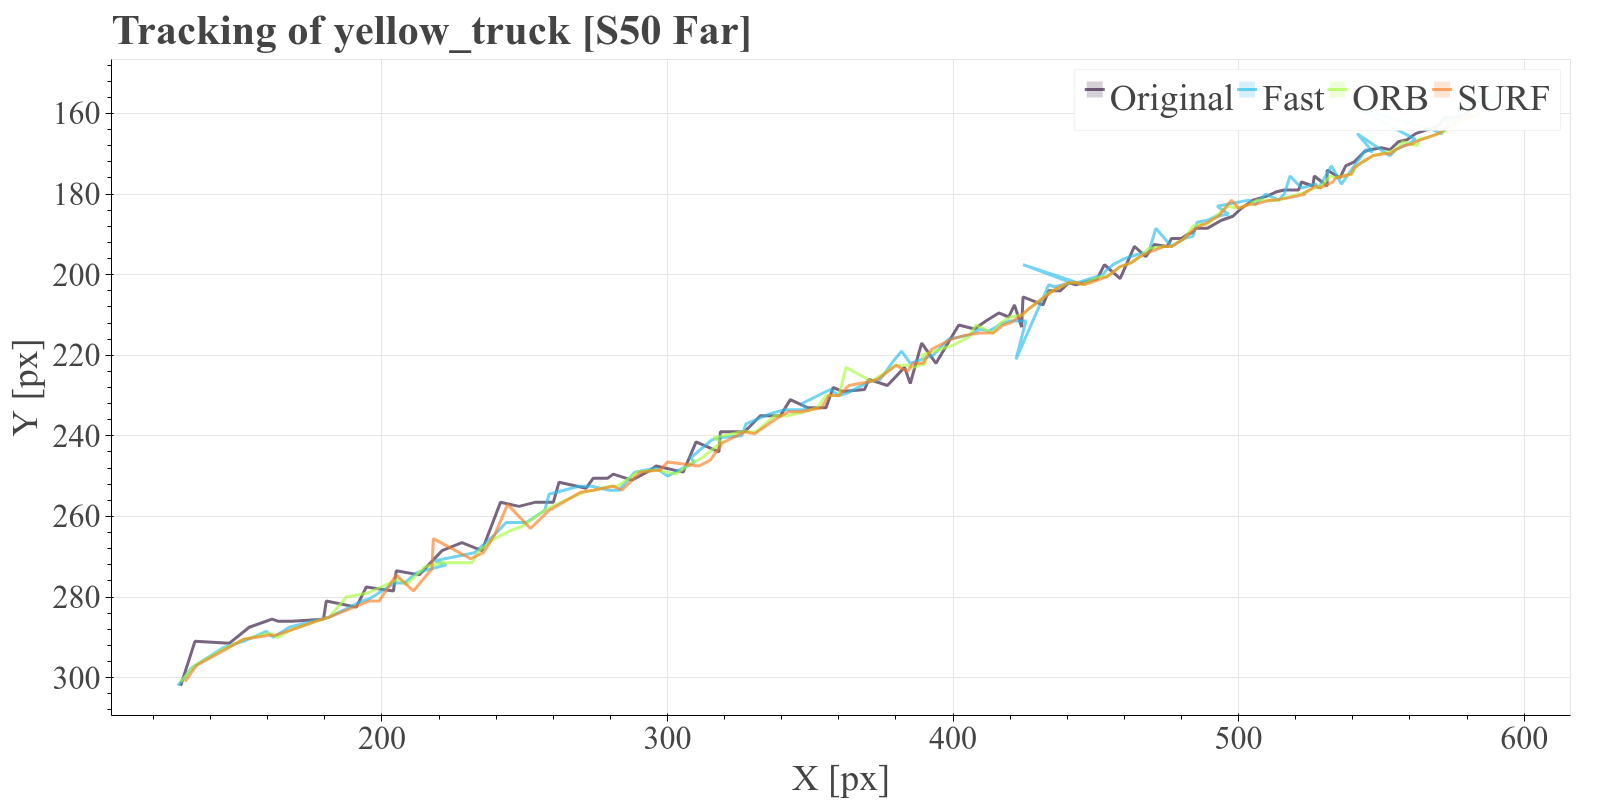
\includegraphics[width=0.475\linewidth]{diagrams/object_tracking/s50_s_far/yellow_truck.png}   
  \end{tabular}
  \caption{Left: 
  The exemplary vehicles tracked through the video sequence of the camera \camsn{4}. 
  Right:
  The corresponding normalized arc lengths of the pixel path. 
  The length is normalized by the original arc length, hence the 1.0 factor for the original video. 
  As the jitter is removed, the pixels movement is lowered significantly as it does only move with the vehicle, not the camera.
  This can be seen with around half of the path length remaining after stabilization for all stabilizers.
  }
  \label{fig:object_tracking_appendix_s50_s_far}
\end{figure*}



\begin{figure*}[!ht]
  \centering
  \begin{tabular}{cc}
    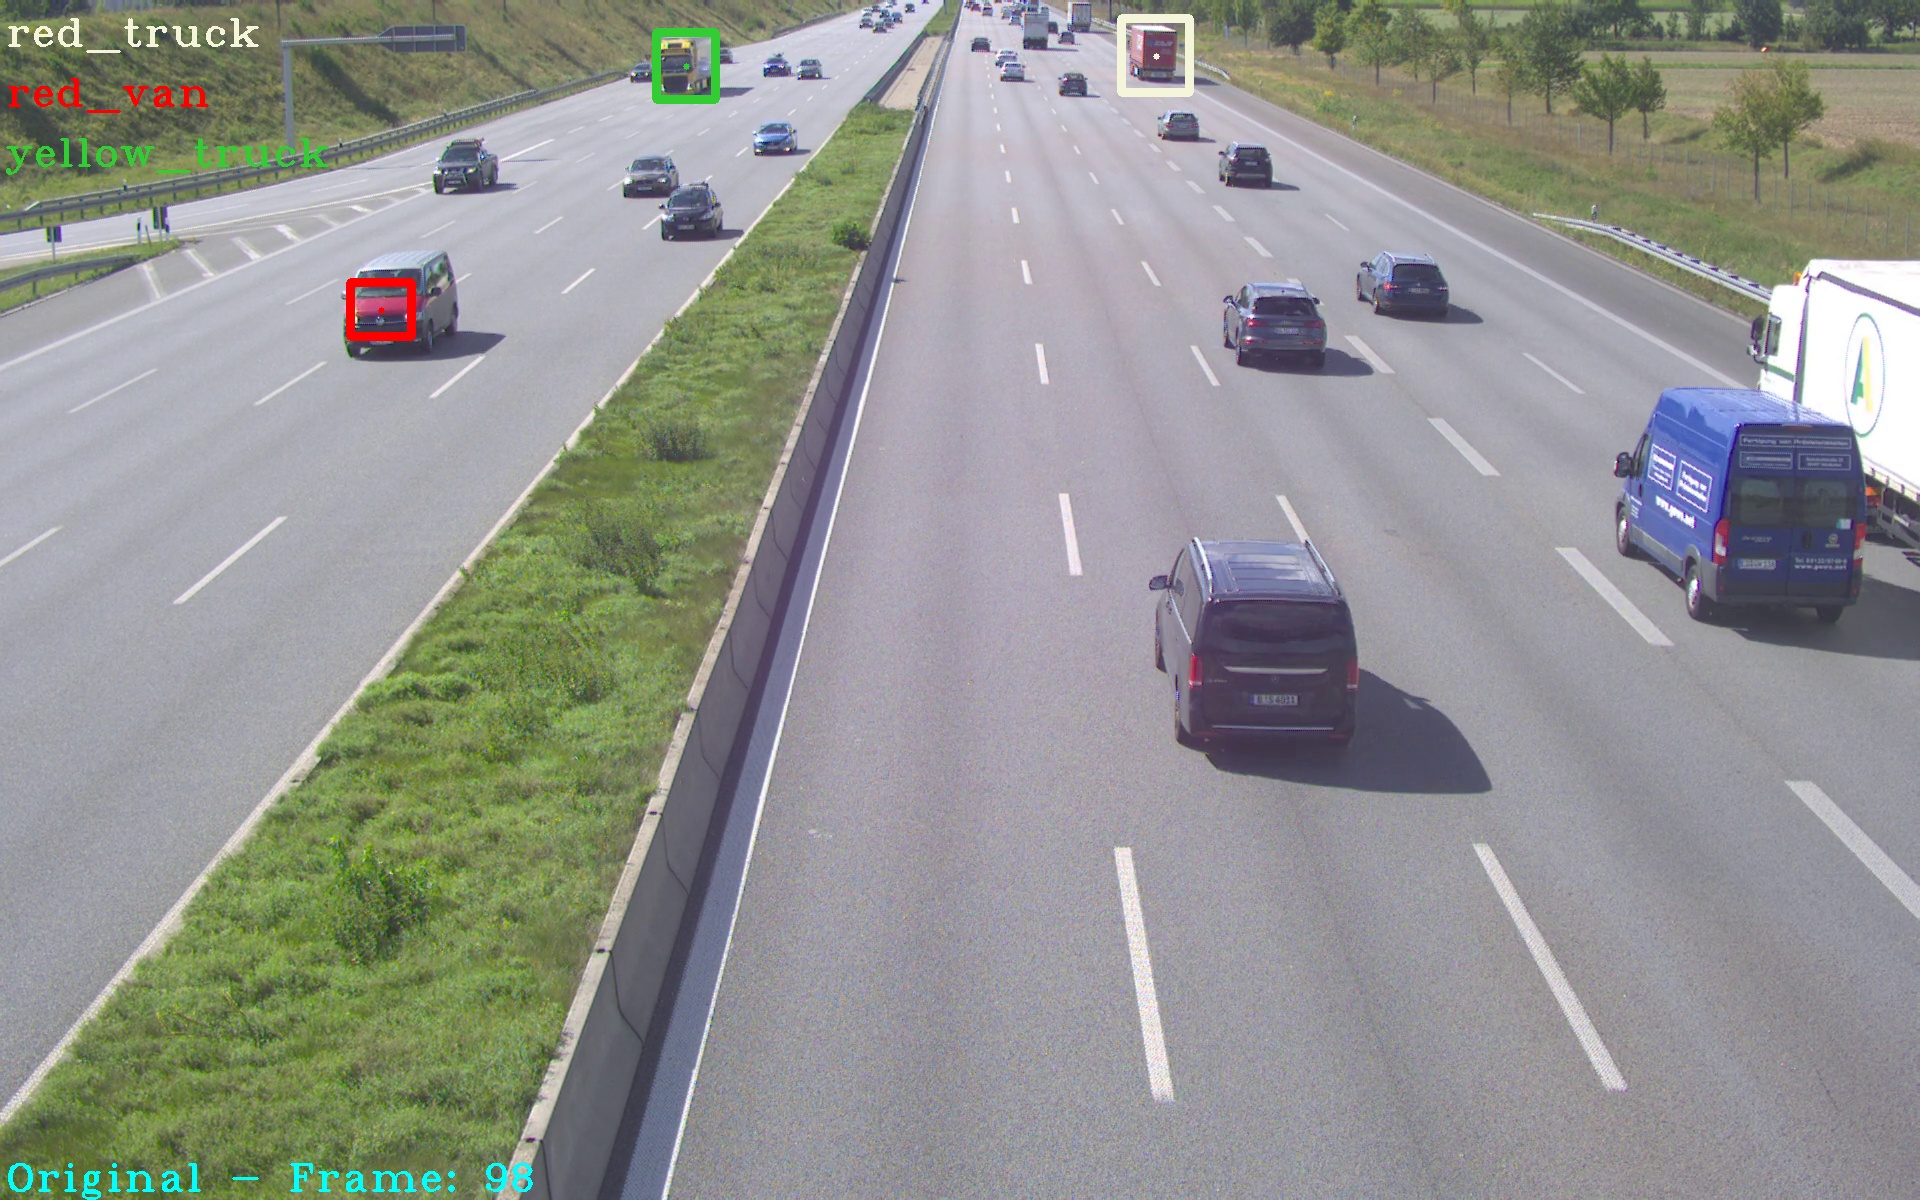
\includegraphics[width=0.45\linewidth]{diagrams/object_tracking/s50_s_near/frame.png}    &  
    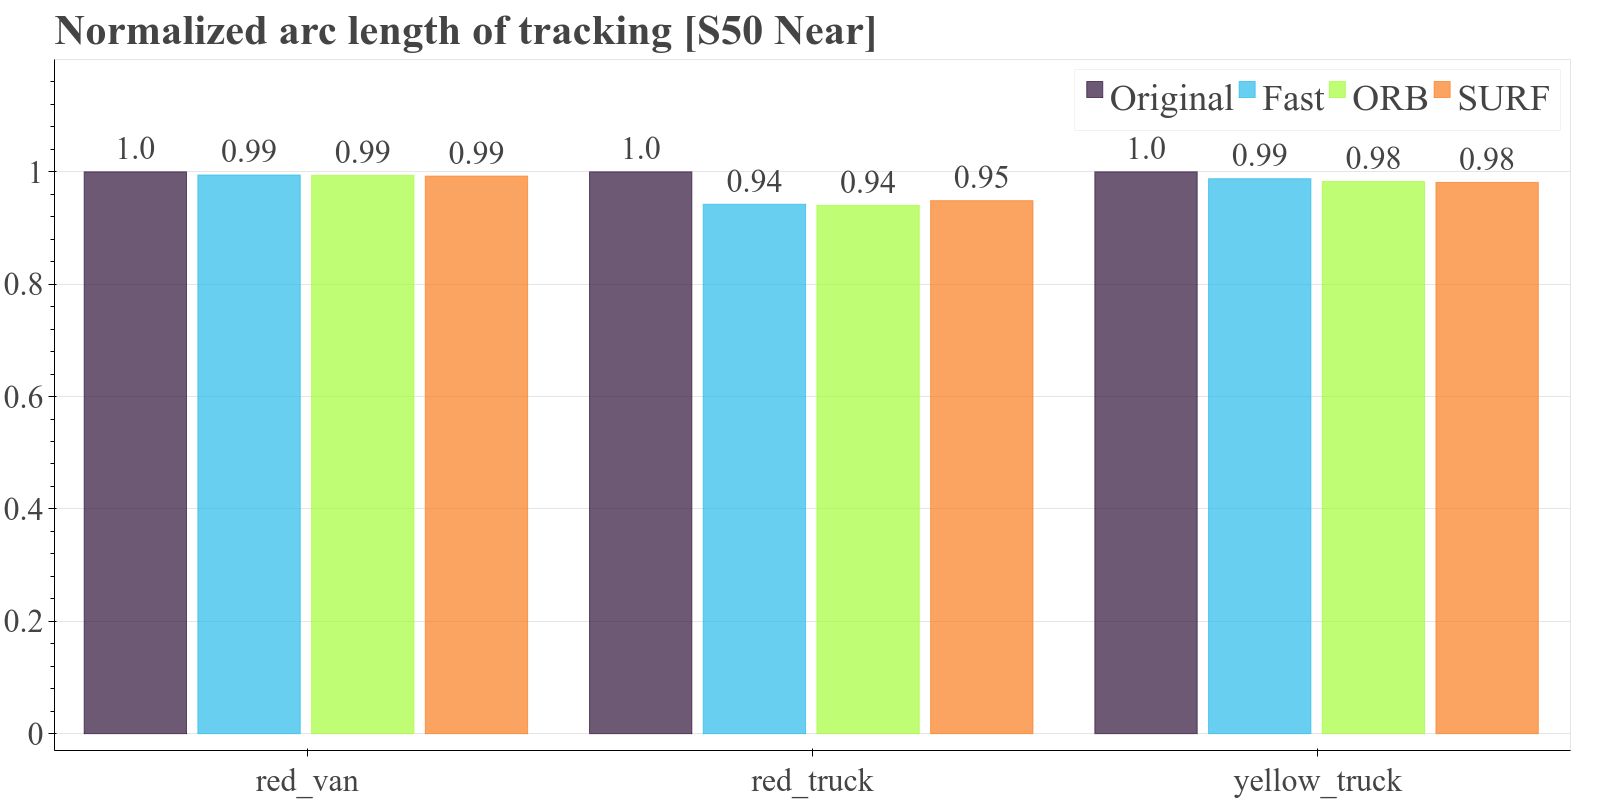
\includegraphics[width=0.475\linewidth]{diagrams/object_tracking/s50_s_near/arcs.png}    \\

    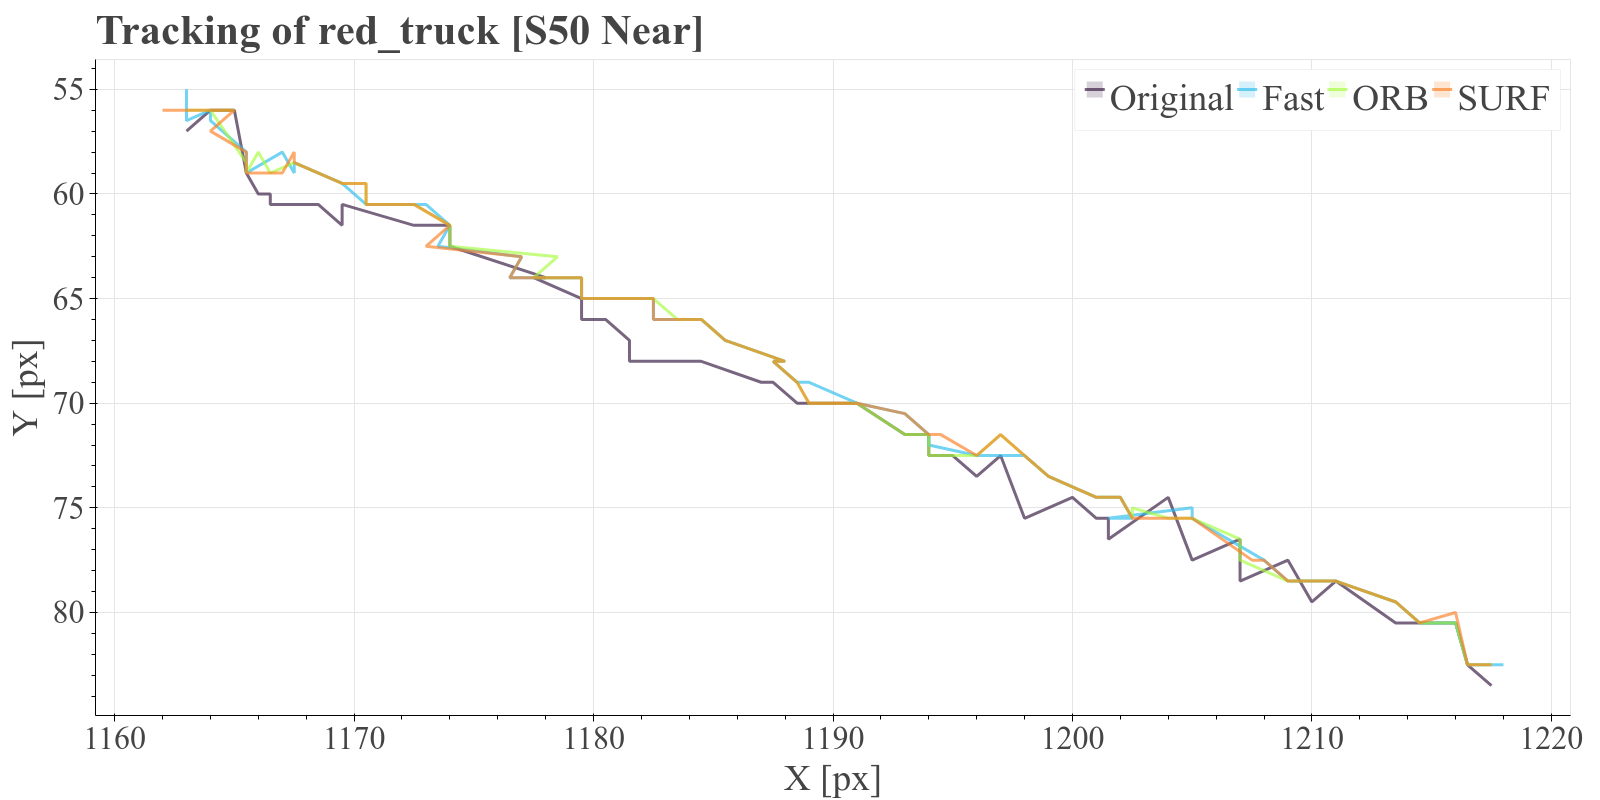
\includegraphics[width=0.475\linewidth]{diagrams/object_tracking/s50_s_near/red_truck.png}    &  
    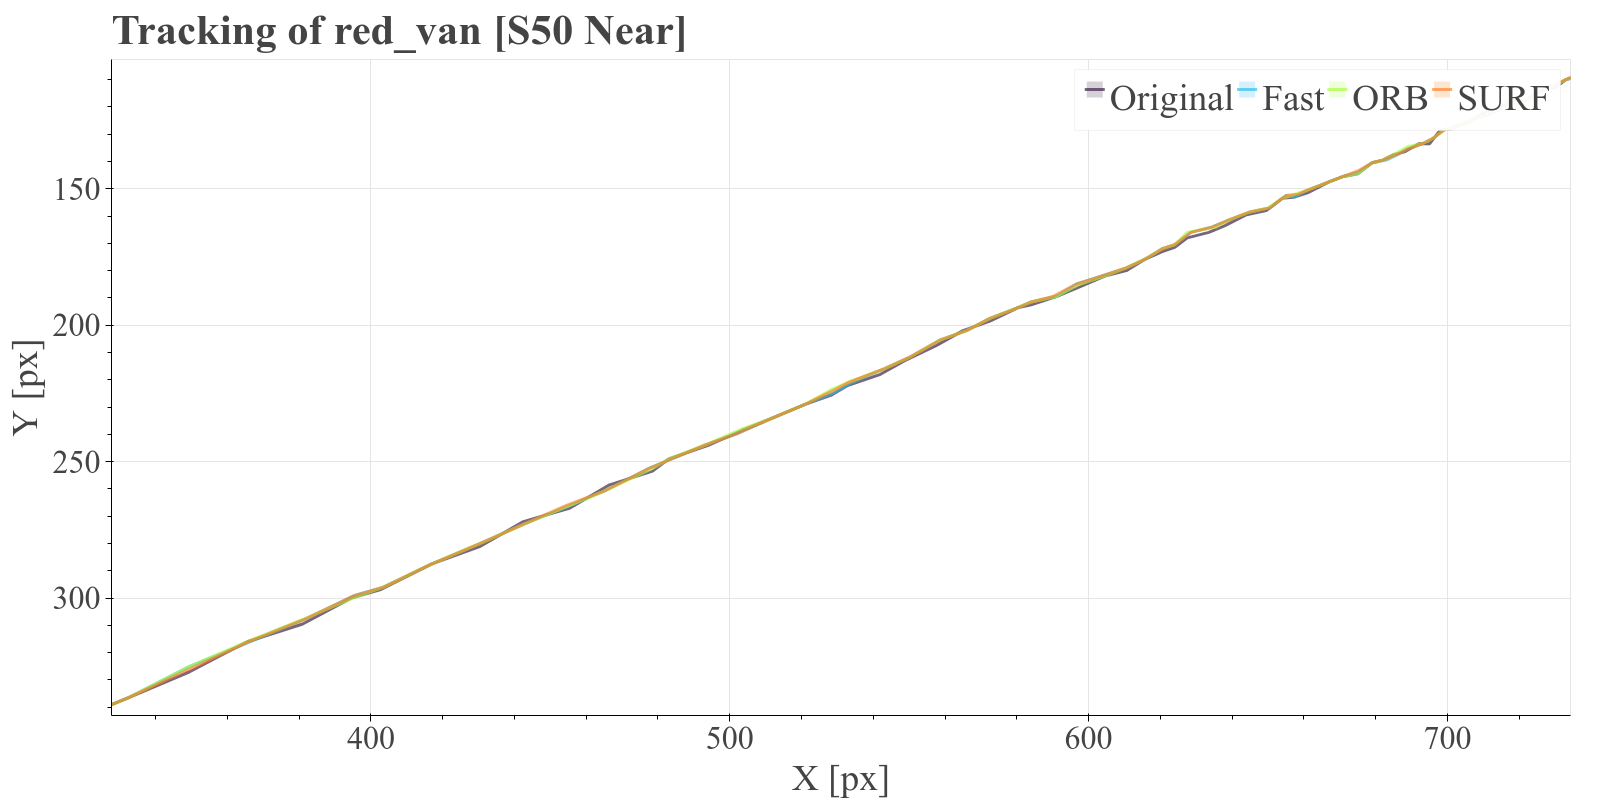
\includegraphics[width=0.475\linewidth]{diagrams/object_tracking/s50_s_near/red_van.png}    \\  
    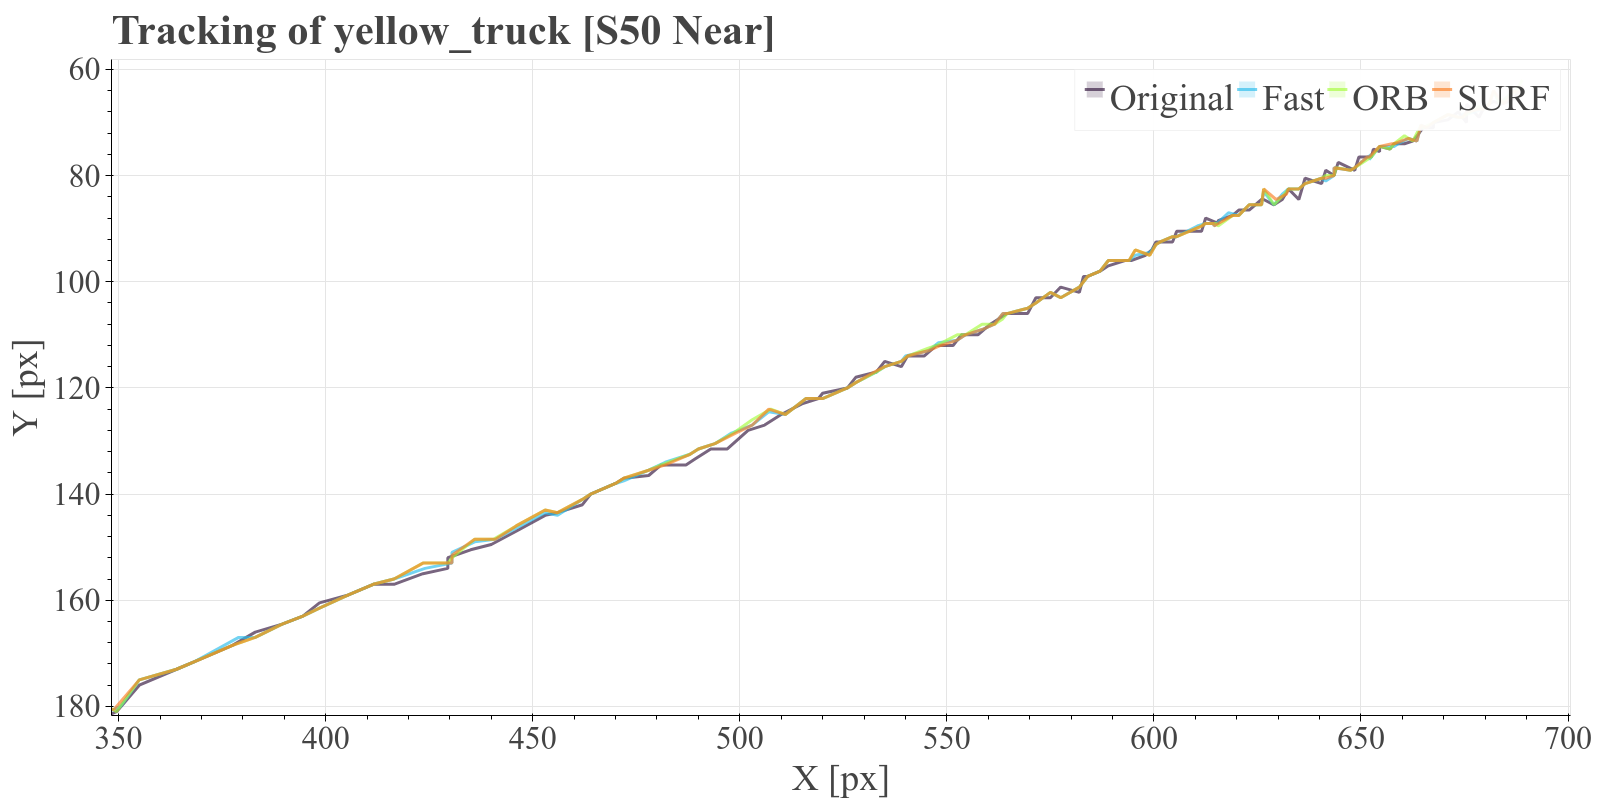
\includegraphics[width=0.475\linewidth]{diagrams/object_tracking/s50_s_near/yellow_truck.png}   
  \end{tabular}
  \caption{Left: 
  The exemplary vehicles tracked through the video sequence of the camera \camsn{4}. 
  Right:
  The corresponding normalized arc lengths of the pixel path. 
  The length is normalized by the original arc length, hence the 1.0 factor for the original video. 
  As the jitter is removed, the pixels movement is lowered significantly as it does only move with the vehicle, not the camera.
  This can be seen with around half of the path length remaining after stabilization for all stabilizers.
  }
  \label{fig:object_tracking_appendix_s50_s_near}
\end{figure*}

\begin{figure*}[!ht]
  \centering
  \begin{tabular}{cc}
    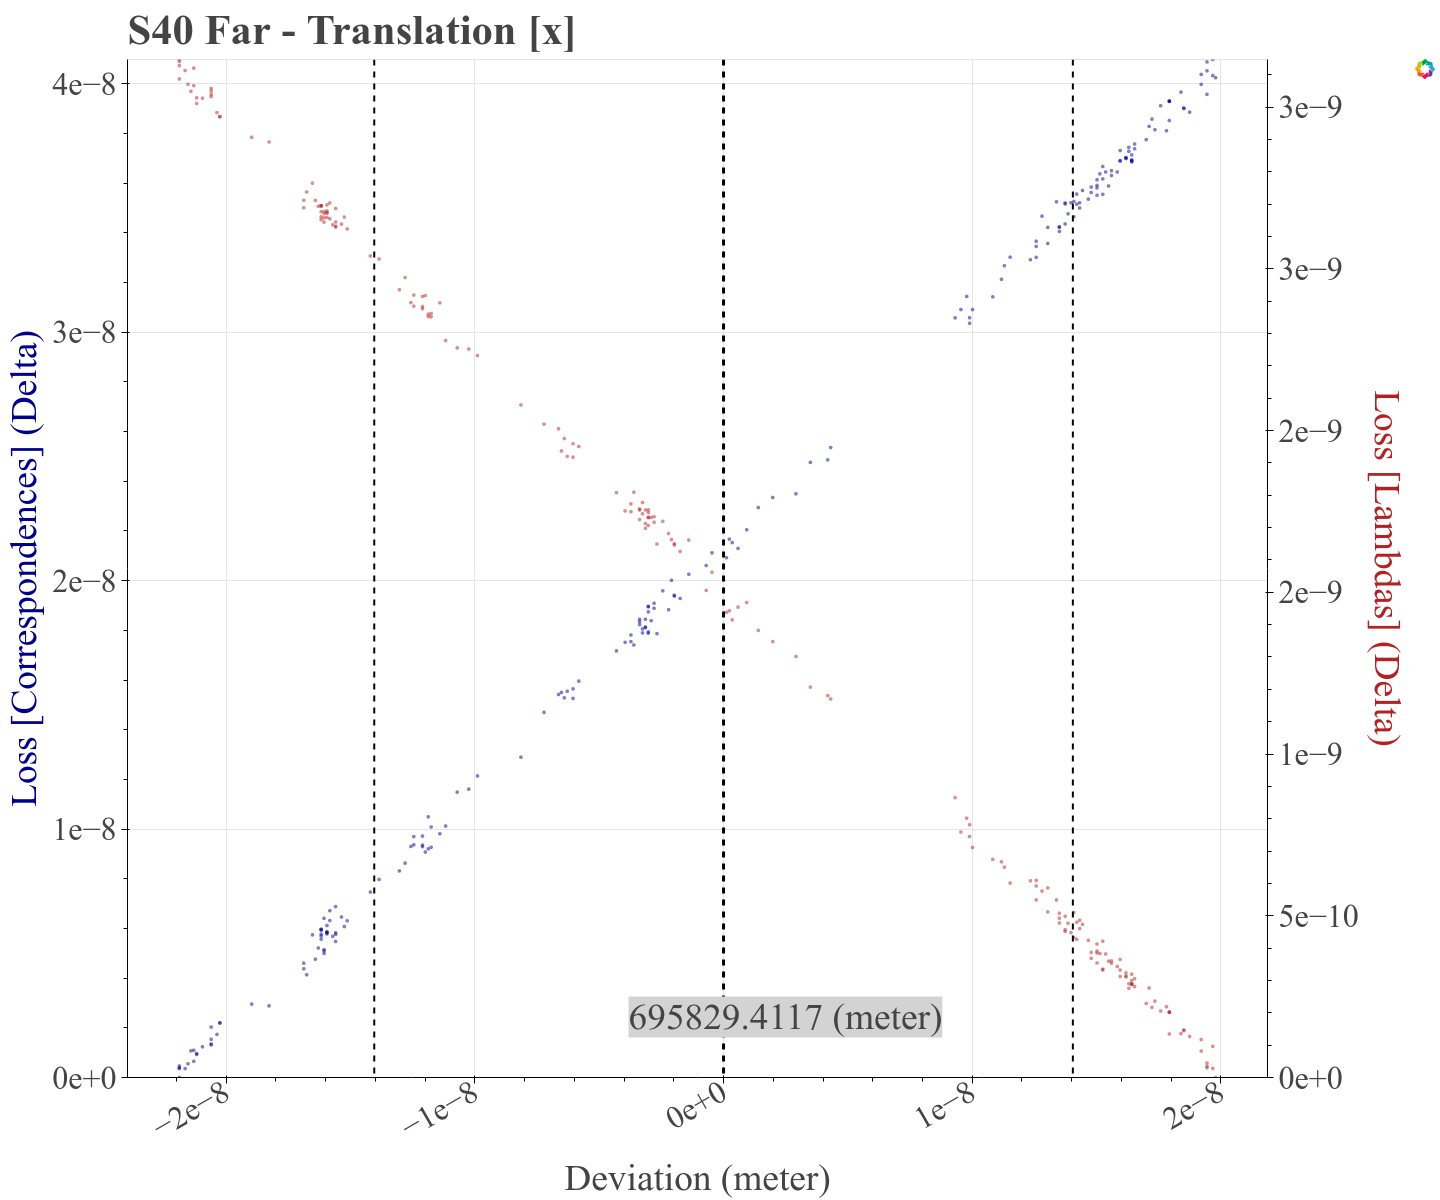
\includegraphics[width=0.45 \linewidth]{diagrams/calibration/s40_n_far/parameters.csv/Translation[x]_vs_Loss[Correspondences]_vs_Loss[Lambdas]_cluster_All.png} &
    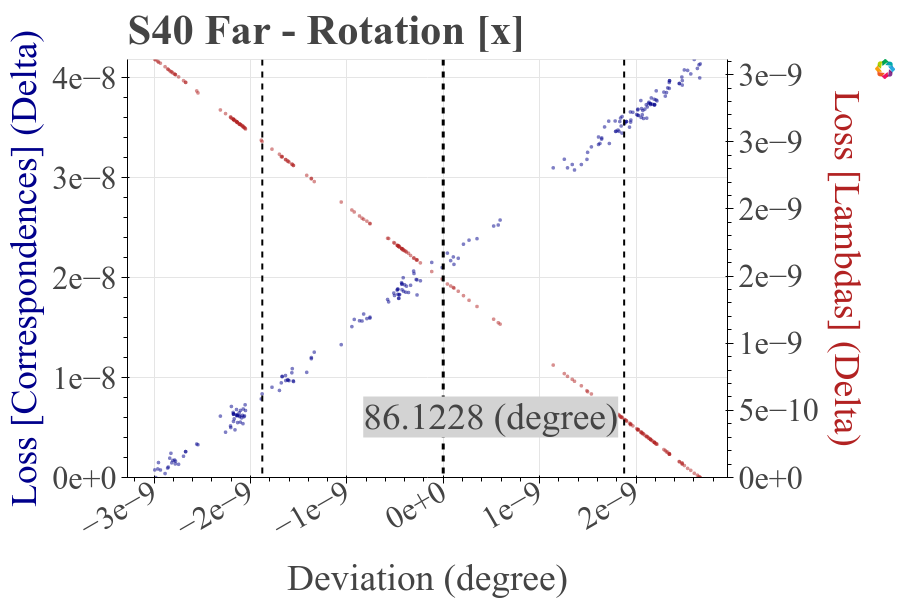
\includegraphics[width=0.45 \linewidth]{diagrams/calibration/s40_n_far/parameters.csv/Rotation[x]_vs_Loss[Correspondences]_vs_Loss[Lambdas]_cluster_All.png} \\
    
    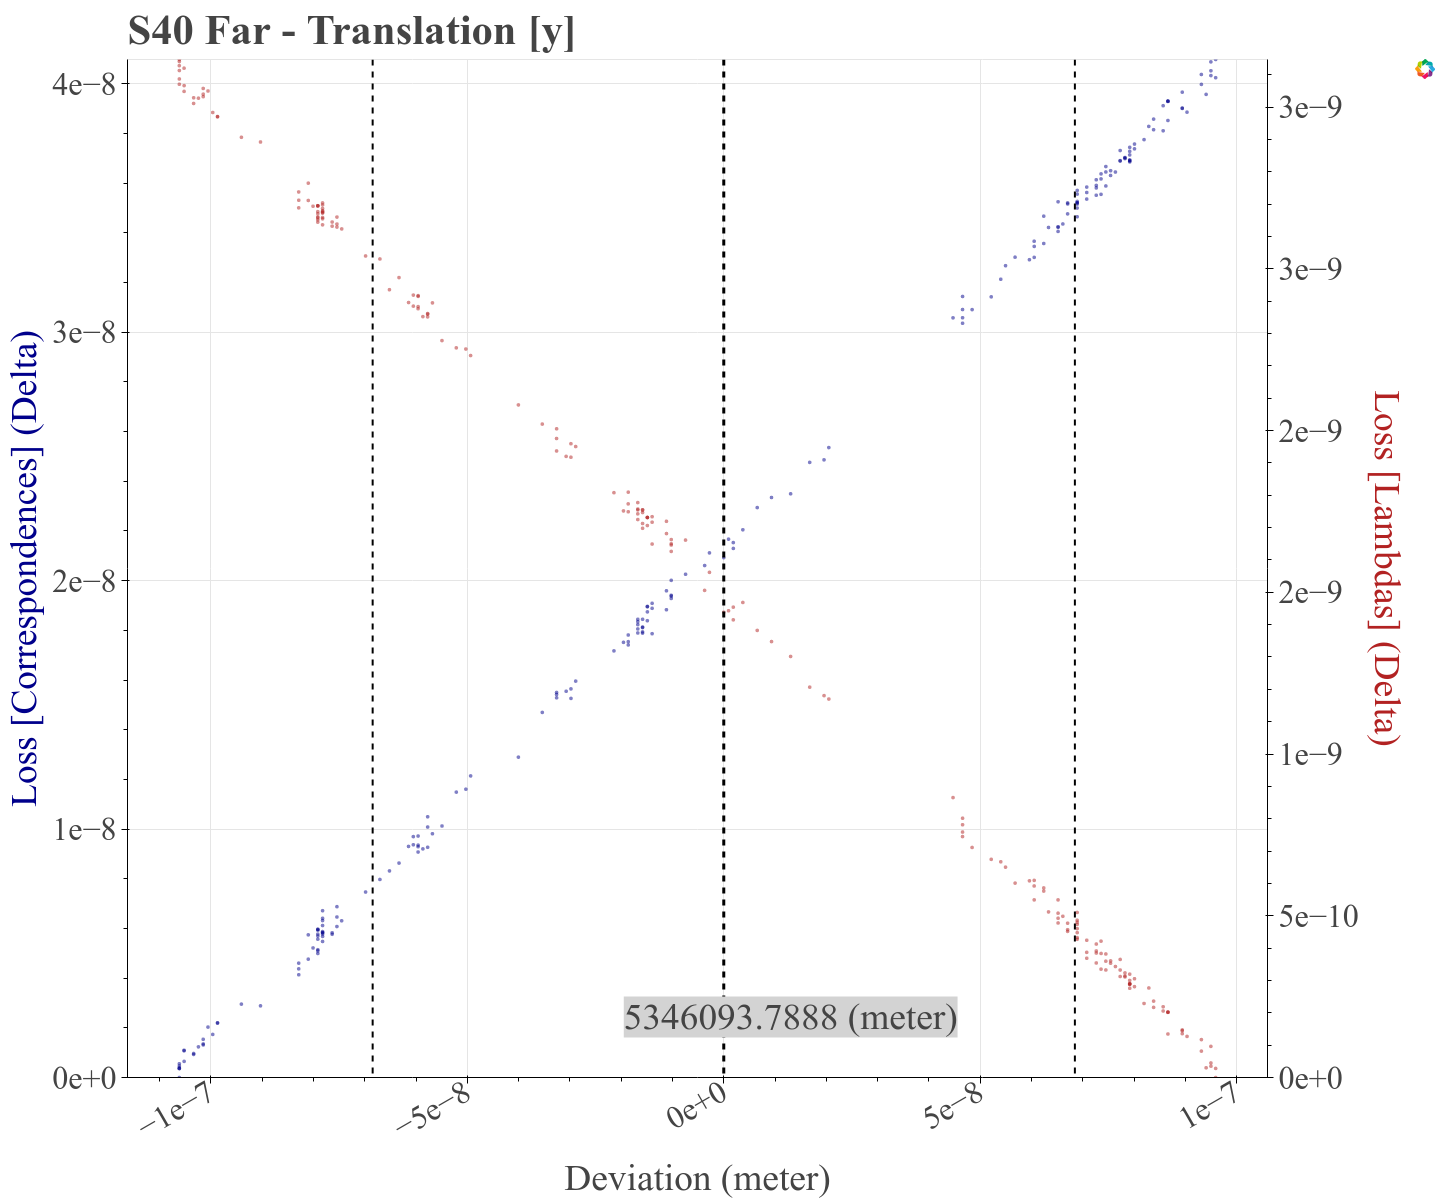
\includegraphics[width=0.45 \linewidth]{diagrams/calibration/s40_n_far/parameters.csv/Translation[y]_vs_Loss[Correspondences]_vs_Loss[Lambdas]_cluster_All.png} &
    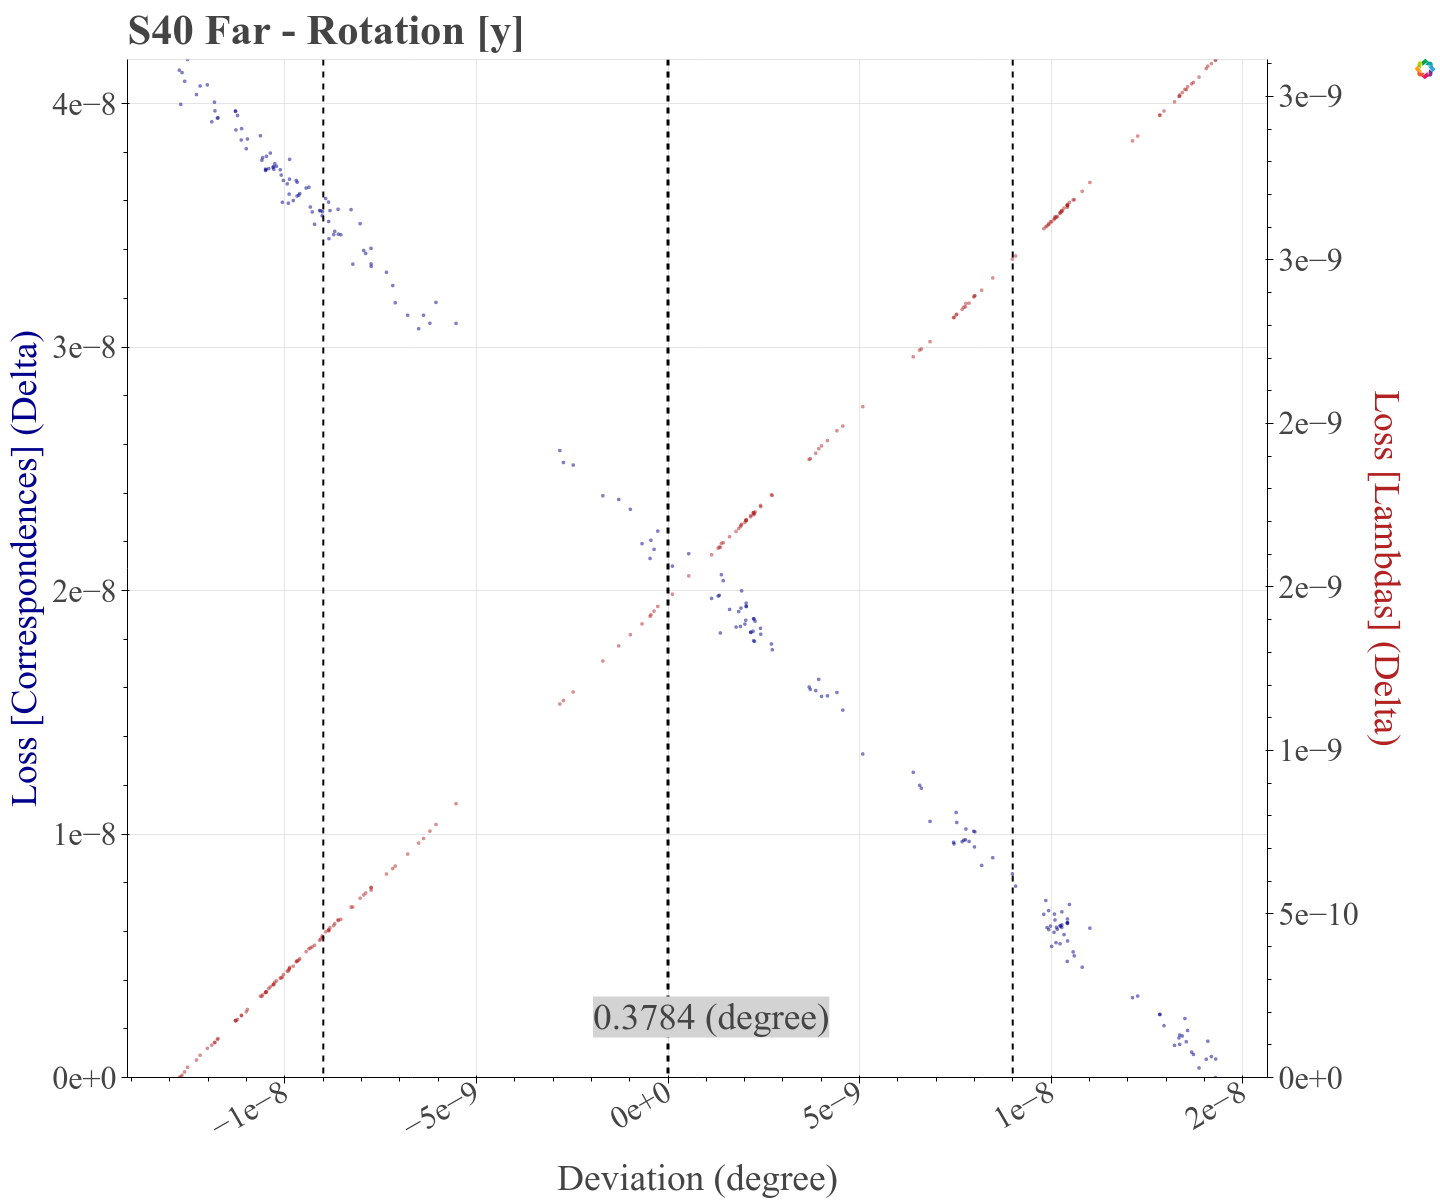
\includegraphics[width=0.45 \linewidth]{diagrams/calibration/s40_n_far/parameters.csv/Rotation[y]_vs_Loss[Correspondences]_vs_Loss[Lambdas]_cluster_All.png} \\
    
    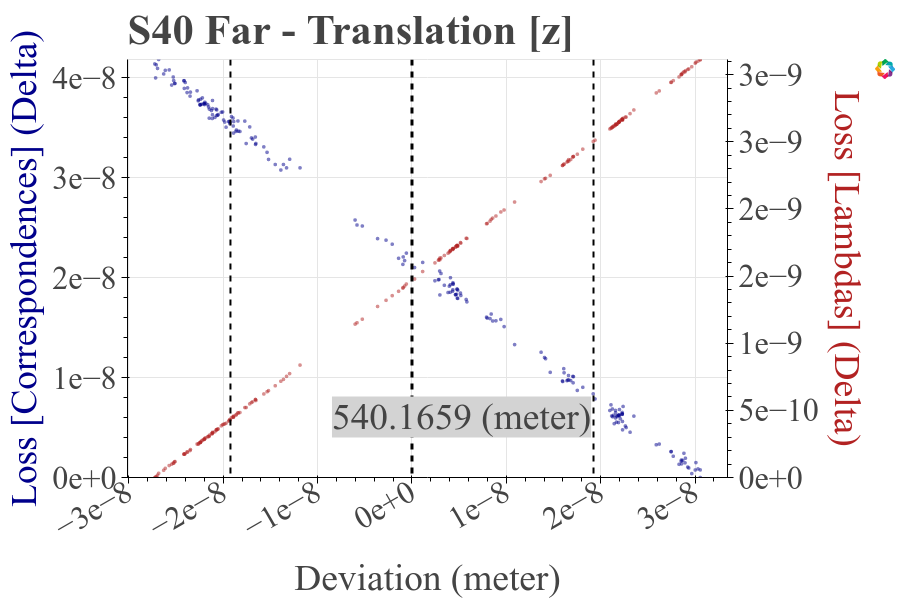
\includegraphics[width=0.45 \linewidth]{diagrams/calibration/s40_n_far/parameters.csv/Translation[z]_vs_Loss[Correspondences]_vs_Loss[Lambdas]_cluster_All.png} &
    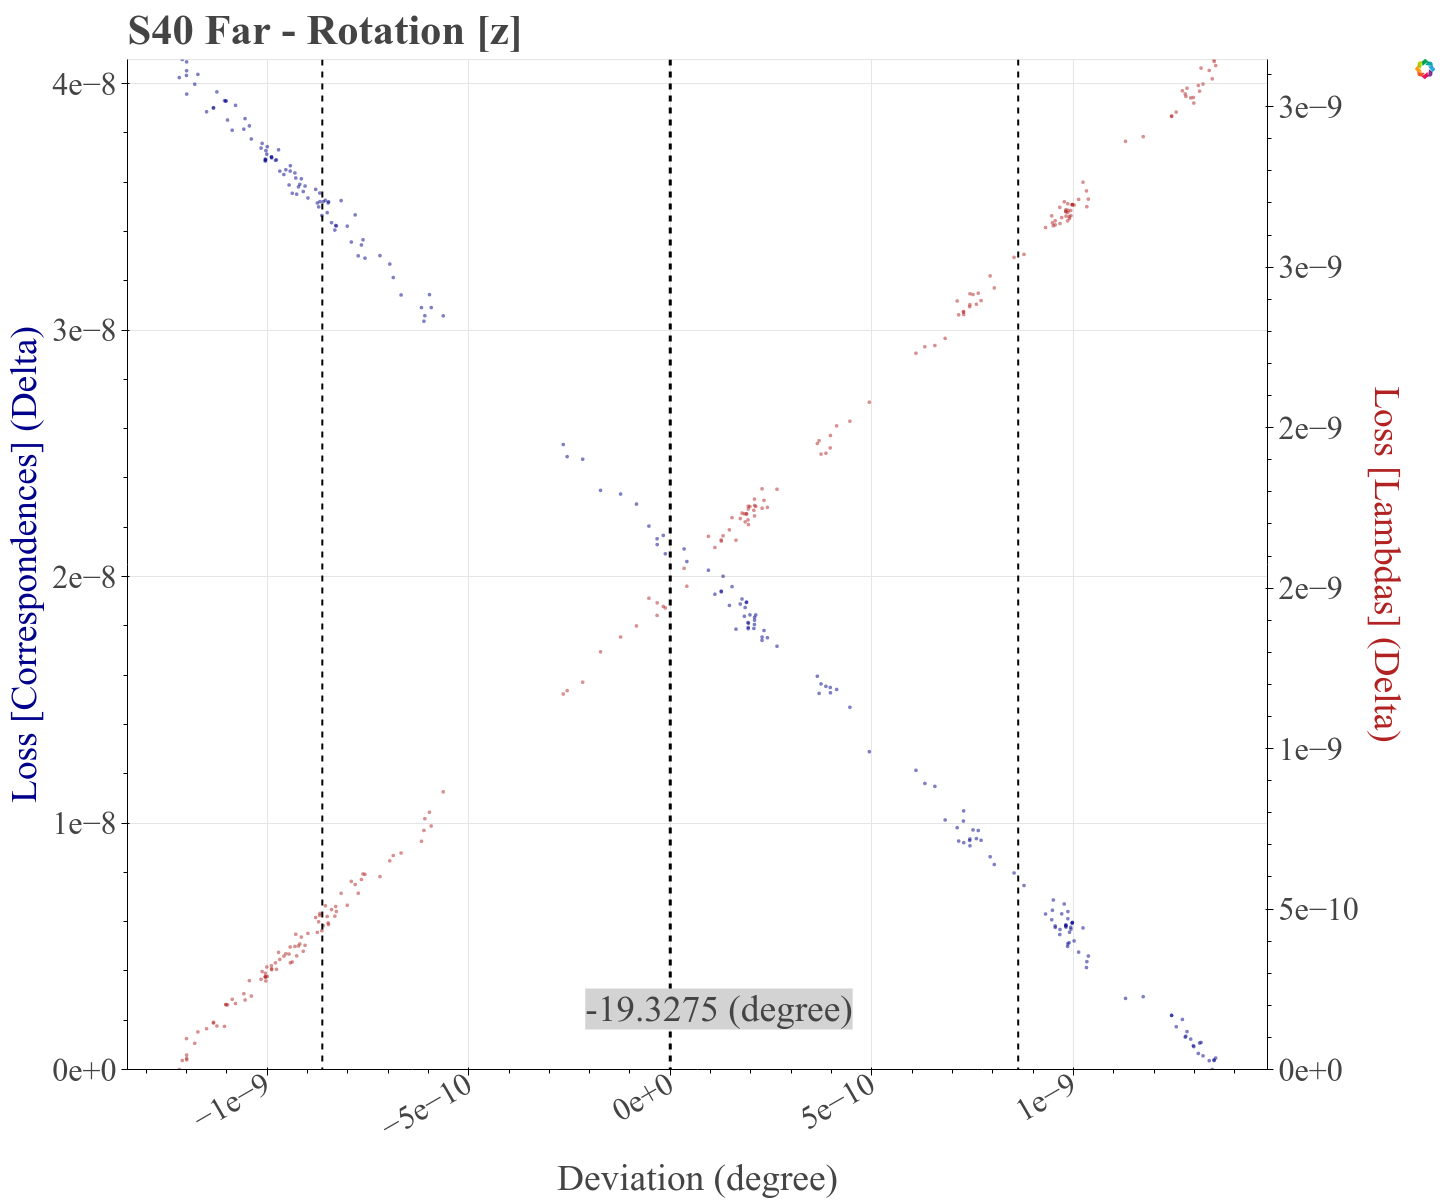
\includegraphics[width=0.45 \linewidth]{diagrams/calibration/s40_n_far/parameters.csv/Rotation[z]_vs_Loss[Correspondences]_vs_Loss[Lambdas]_cluster_All.png} \\

    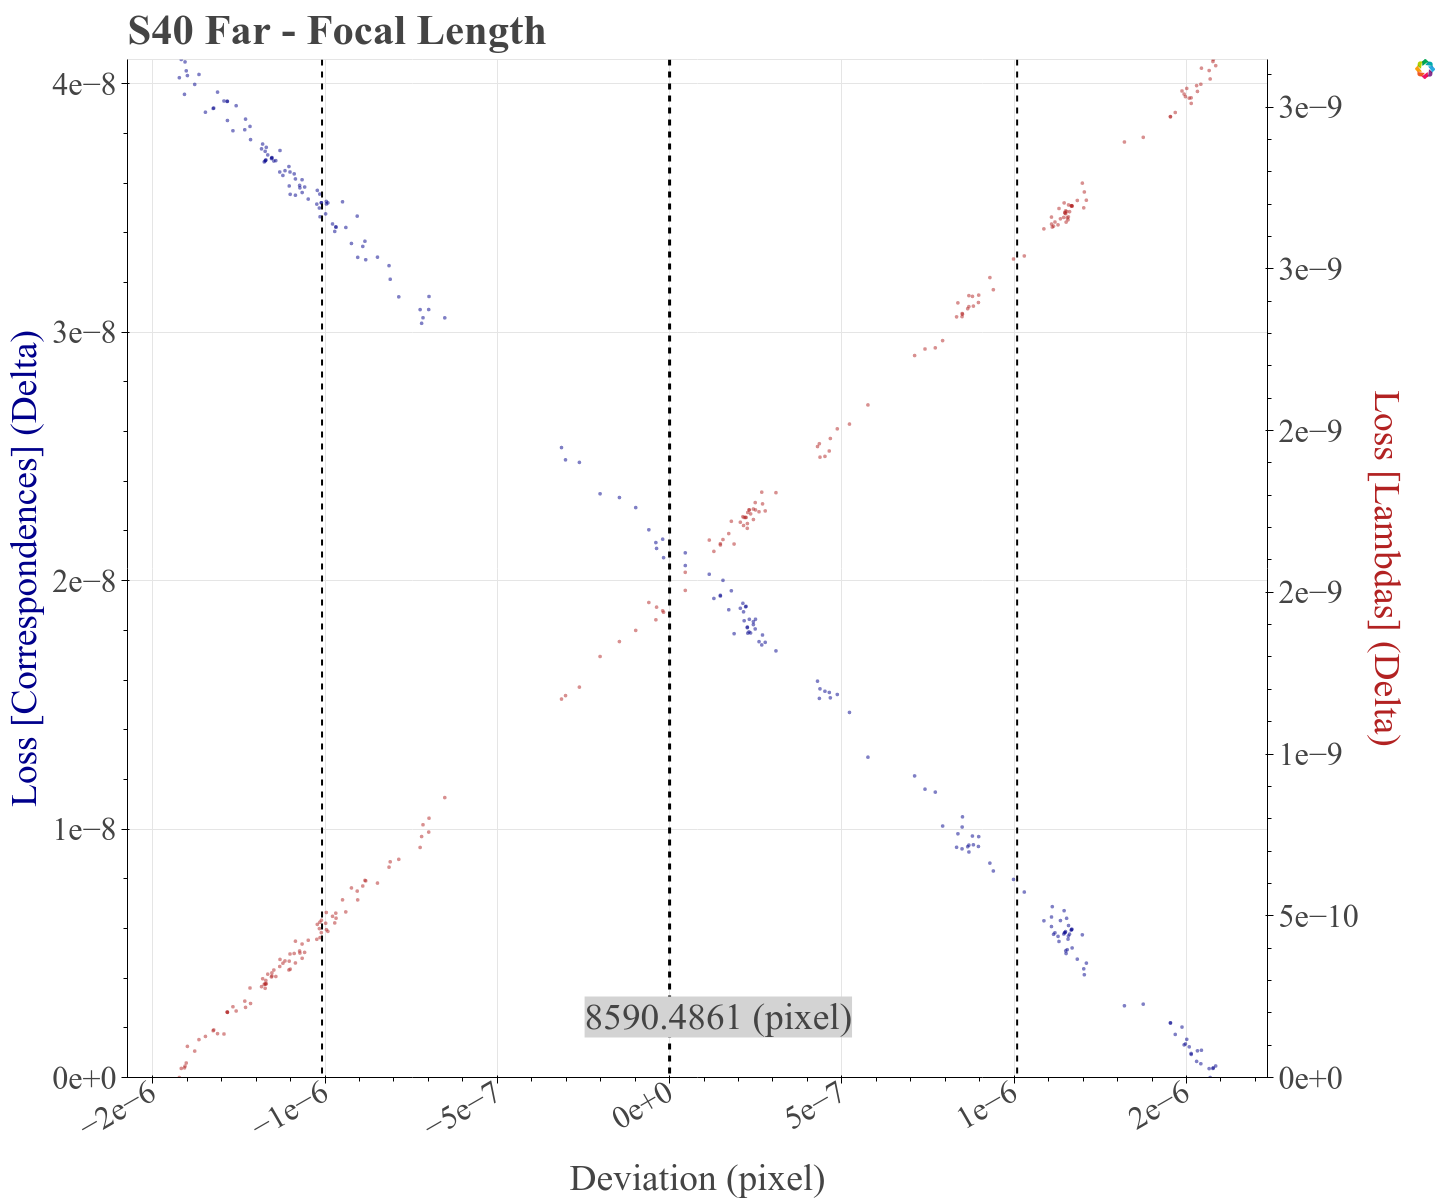
\includegraphics[width=0.45 \linewidth]{diagrams/calibration/s40_n_far/parameters.csv/FocalLength_vs_Loss[Correspondences]_vs_Loss[Lambdas]_cluster_All.png} &
\end{tabular}
\caption{
  Left: The resulting translational parameters plotted against the remaining losses. 
  Right: The resulting rotational parameters plotted against the remaining losses.
  Bottom: The resulting focal length  plotted against the remaining losses.
   }
\label{fig:static_calibration_algorithmic_error_s40_n_far}
\end{figure*}

\begin{figure*}[!ht]
  \centering
  \begin{tabular}{cc}
    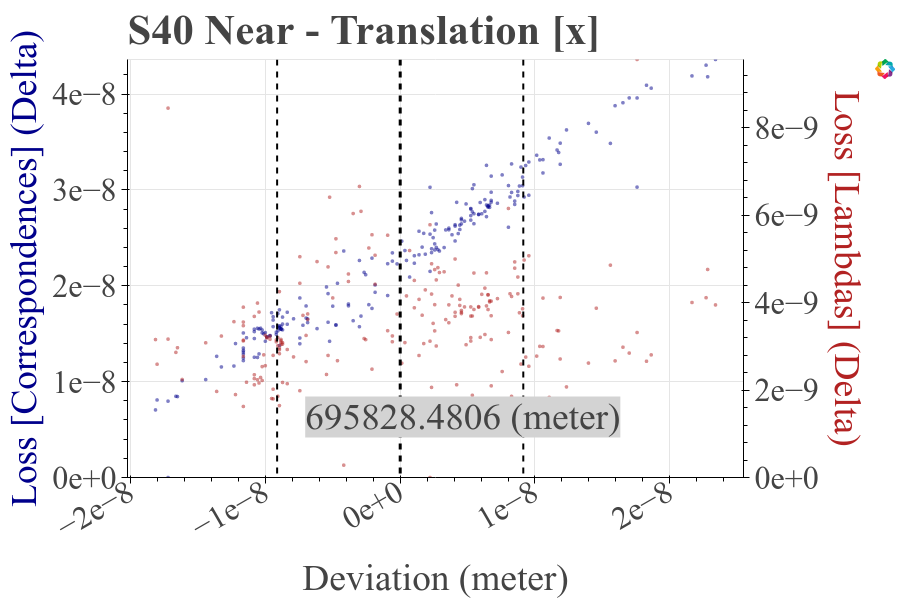
\includegraphics[width=0.45 \linewidth]{diagrams/calibration/s40_n_near/parameters.csv/Translation[x]_vs_Loss[Correspondences]_vs_Loss[Lambdas]_cluster_All.png} &
    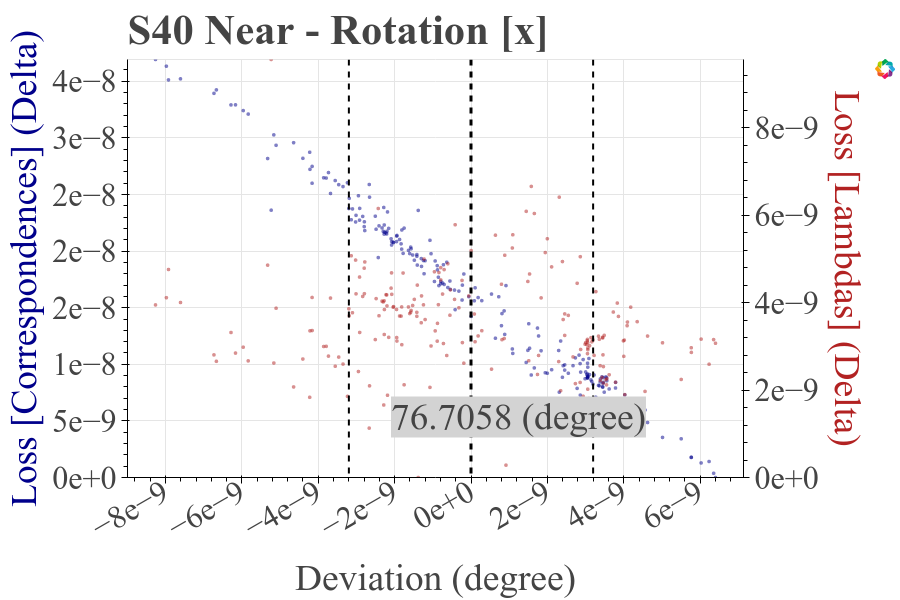
\includegraphics[width=0.45 \linewidth]{diagrams/calibration/s40_n_near/parameters.csv/Rotation[x]_vs_Loss[Correspondences]_vs_Loss[Lambdas]_cluster_All.png} \\
    
    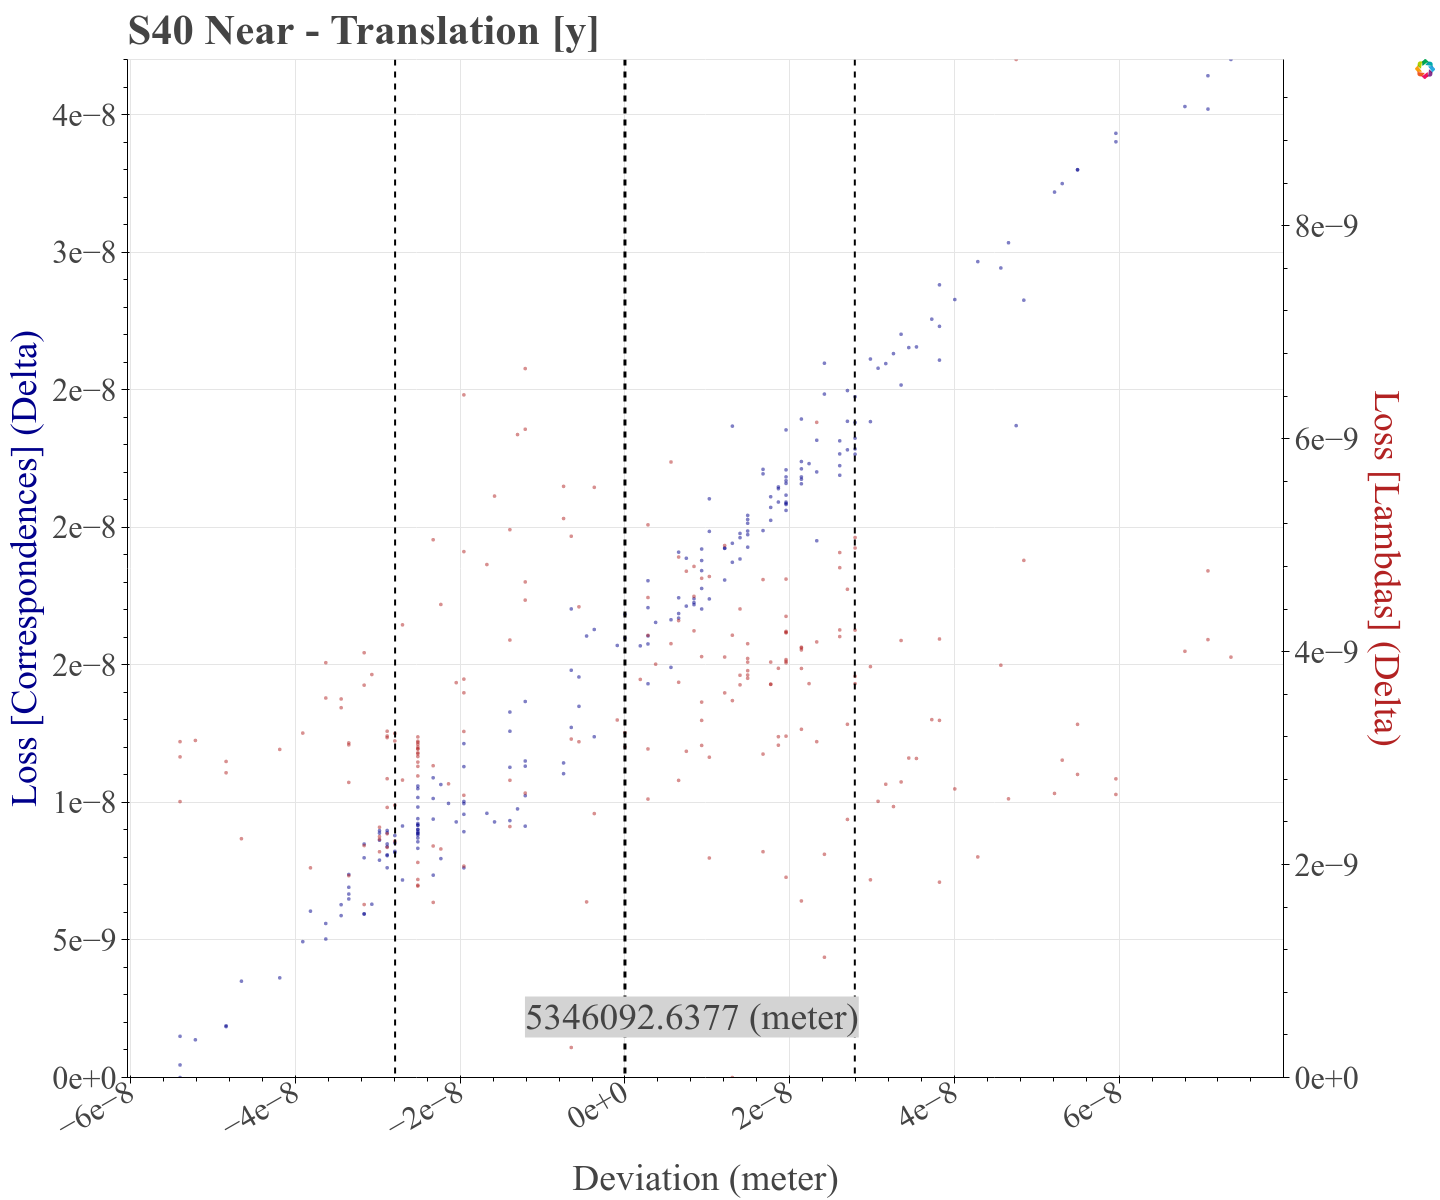
\includegraphics[width=0.45 \linewidth]{diagrams/calibration/s40_n_near/parameters.csv/Translation[y]_vs_Loss[Correspondences]_vs_Loss[Lambdas]_cluster_All.png} &
    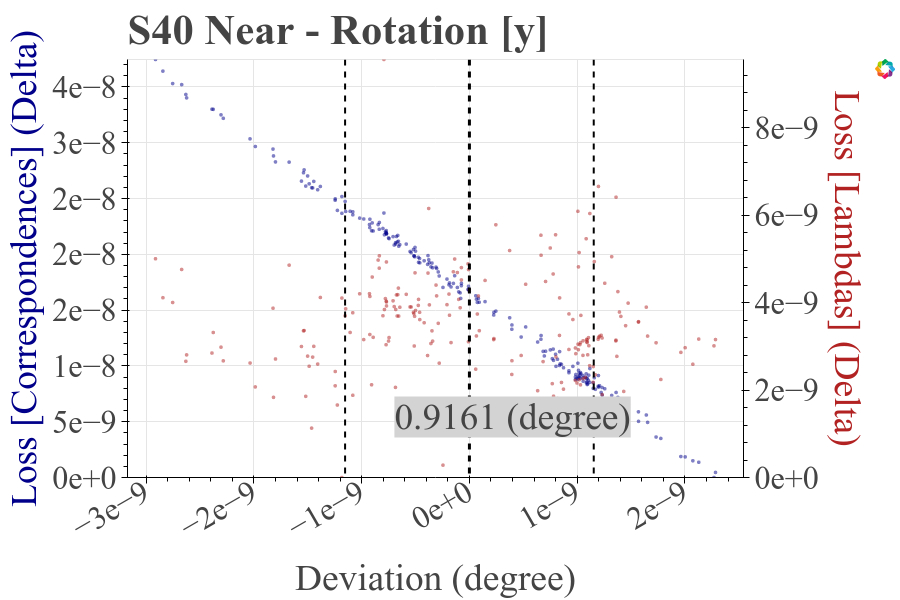
\includegraphics[width=0.45 \linewidth]{diagrams/calibration/s40_n_near/parameters.csv/Rotation[y]_vs_Loss[Correspondences]_vs_Loss[Lambdas]_cluster_All.png} \\
    
    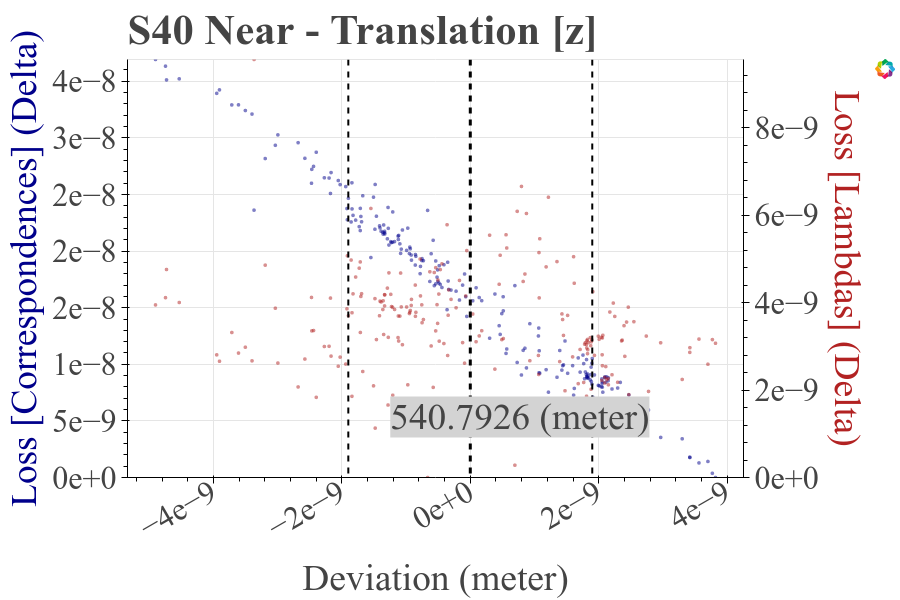
\includegraphics[width=0.45 \linewidth]{diagrams/calibration/s40_n_near/parameters.csv/Translation[z]_vs_Loss[Correspondences]_vs_Loss[Lambdas]_cluster_All.png} &
    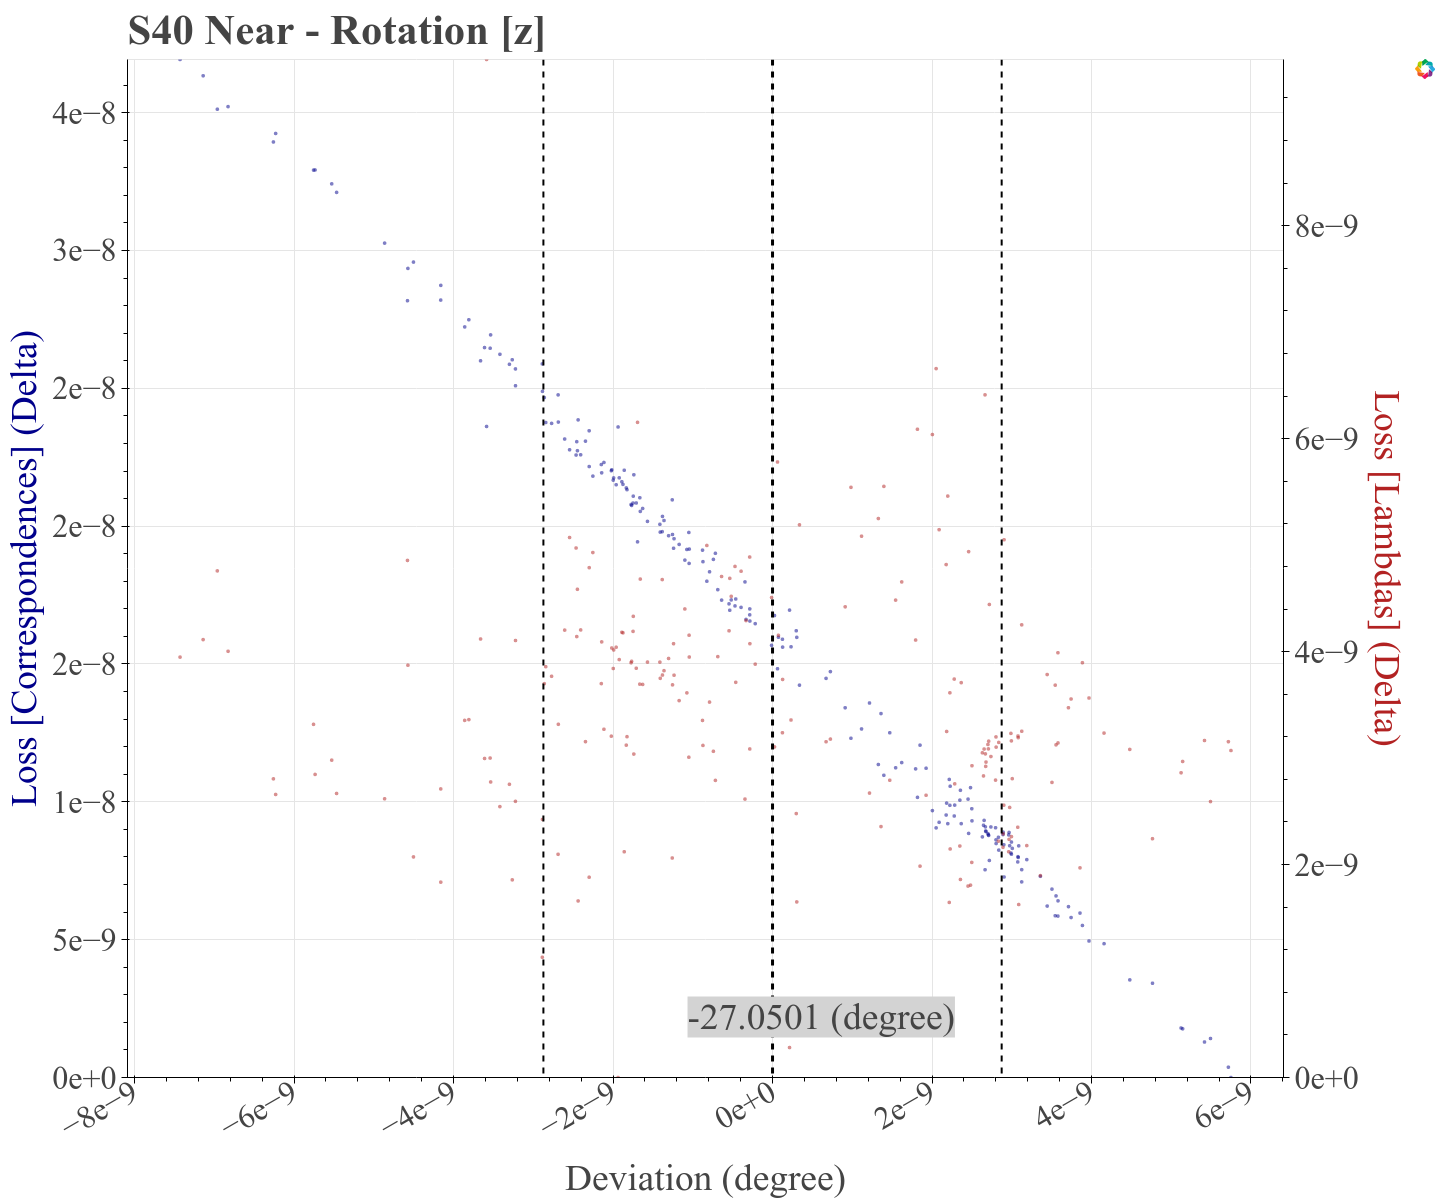
\includegraphics[width=0.45 \linewidth]{diagrams/calibration/s40_n_near/parameters.csv/Rotation[z]_vs_Loss[Correspondences]_vs_Loss[Lambdas]_cluster_All.png} \\

    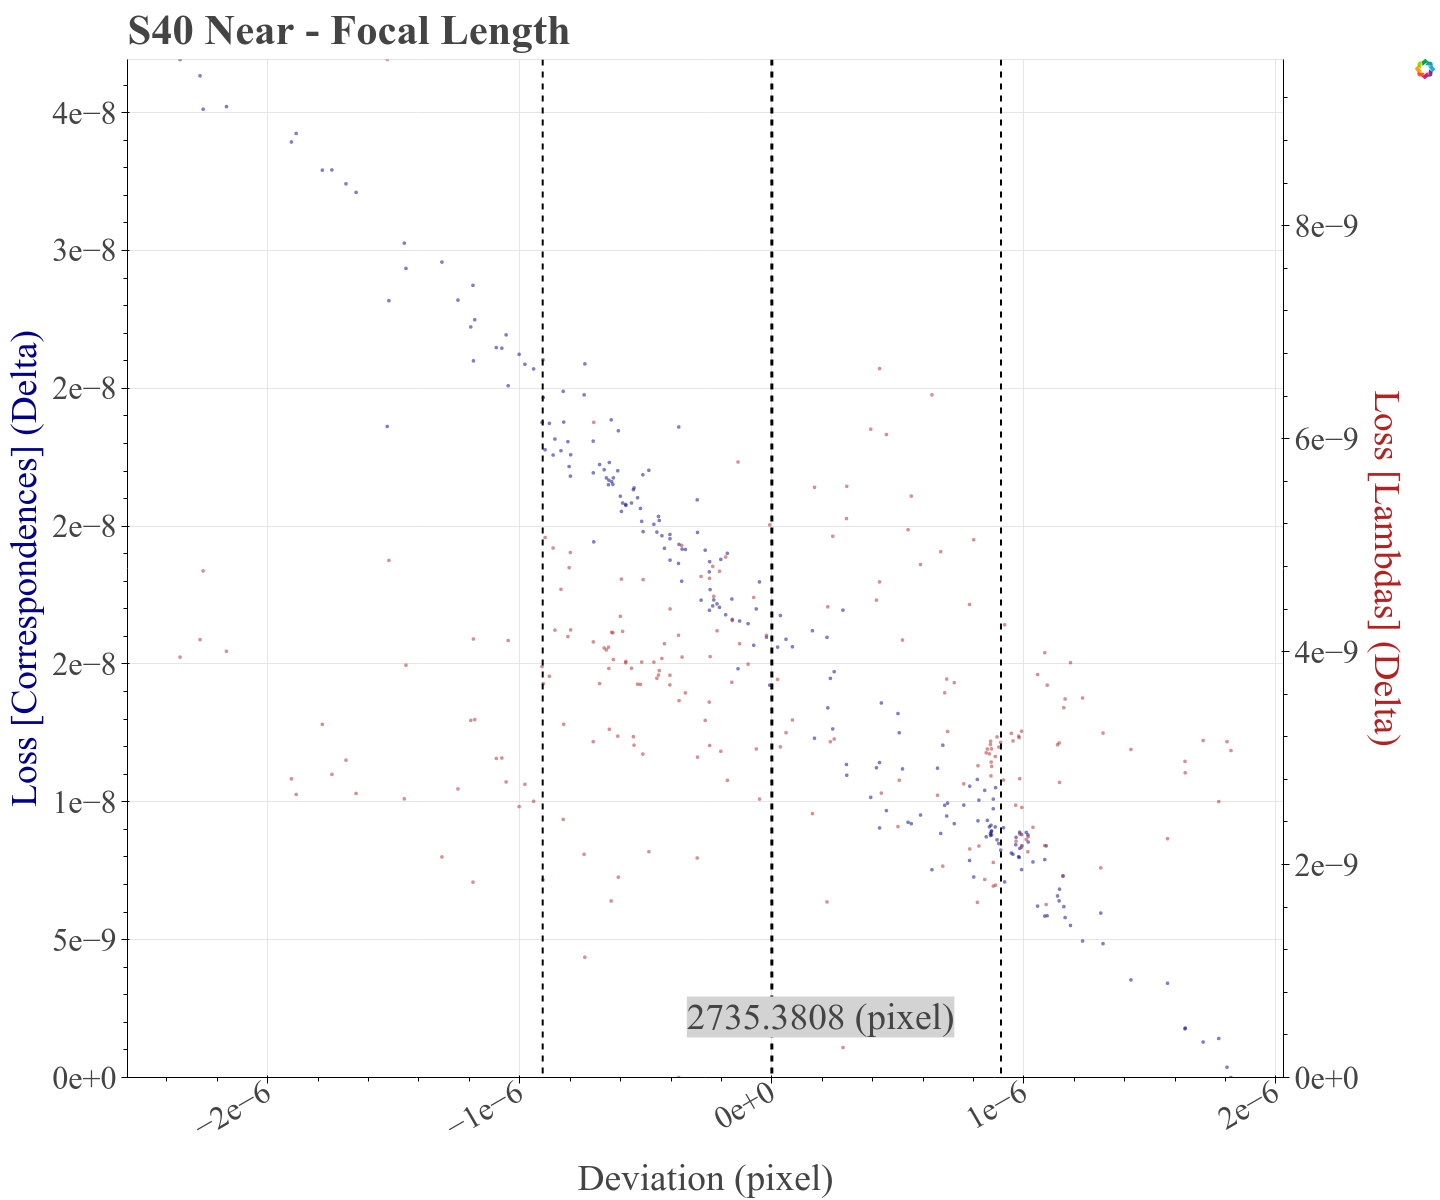
\includegraphics[width=0.45 \linewidth]{diagrams/calibration/s40_n_near/parameters.csv/FocalLength_vs_Loss[Correspondences]_vs_Loss[Lambdas]_cluster_All.png} &
\end{tabular}
\caption{
  Left: The resulting translational parameters plotted against the remaining losses. 
  Right: The resulting rotational parameters plotted against the remaining losses.
  Bottom: The resulting focal length  plotted against the remaining losses.
     }
\label{fig:static_calibration_algorithmic_error_s40_n_near}
\end{figure*}

\begin{figure*}[!ht]
  \centering
  \begin{tabular}{cc}
    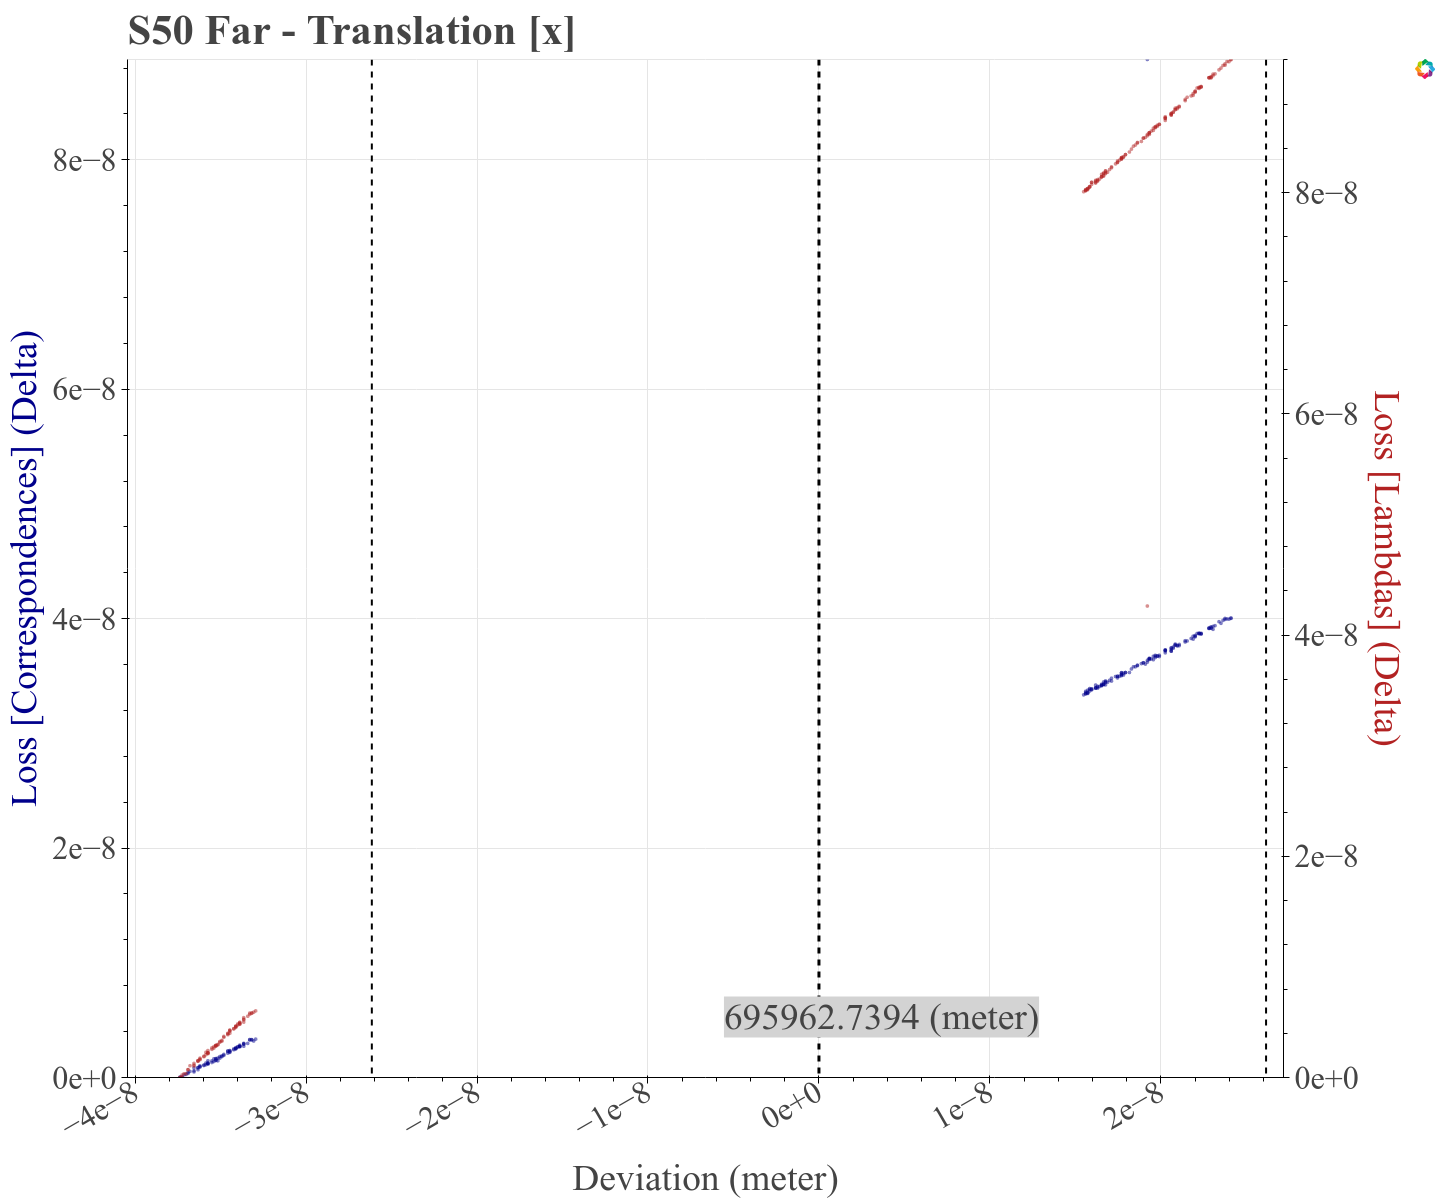
\includegraphics[width=0.45 \linewidth]{diagrams/calibration/s50_s_far/parameters.csv/Translation[x]_vs_Loss[Correspondences]_vs_Loss[Lambdas]_cluster_All.png} &
    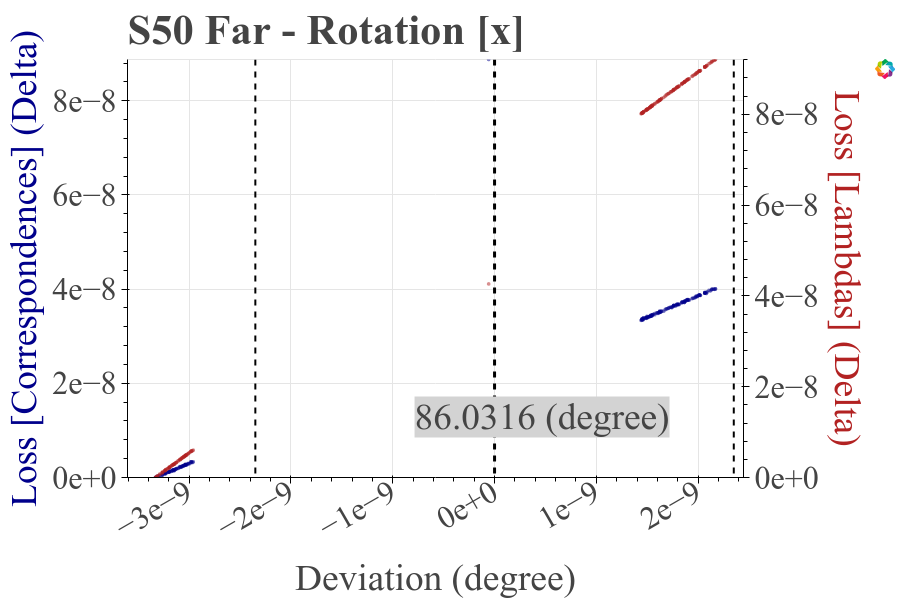
\includegraphics[width=0.45 \linewidth]{diagrams/calibration/s50_s_far/parameters.csv/Rotation[x]_vs_Loss[Correspondences]_vs_Loss[Lambdas]_cluster_All.png} \\
    
    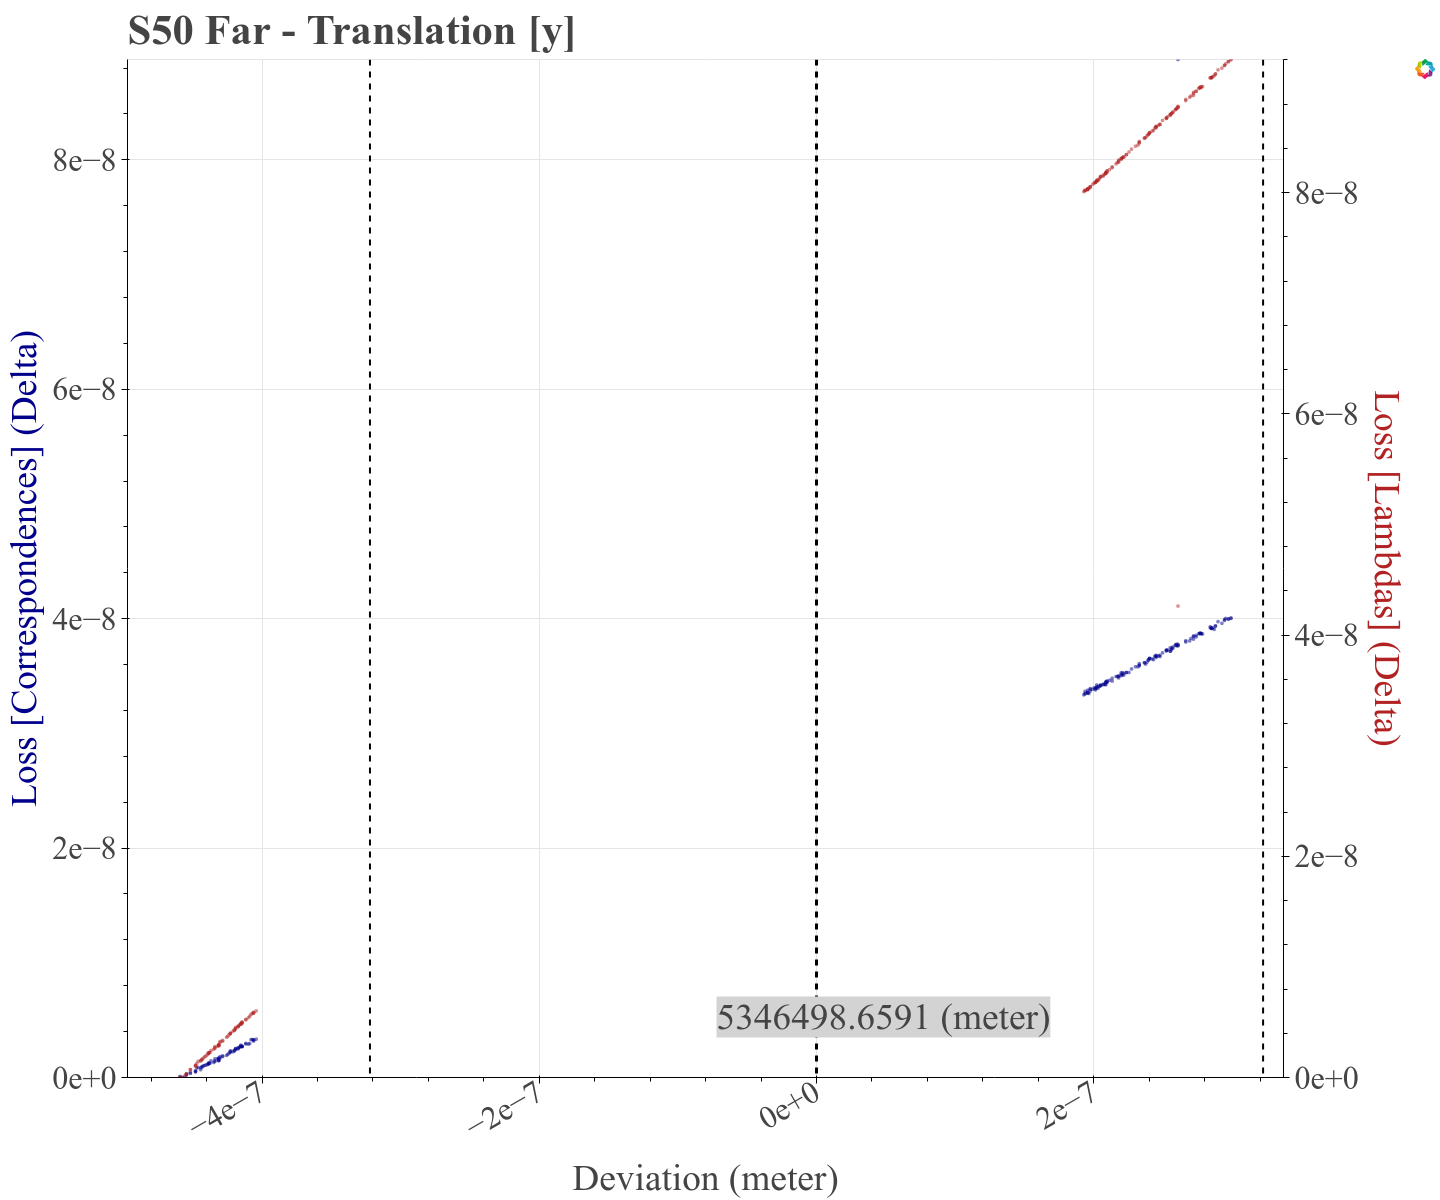
\includegraphics[width=0.45 \linewidth]{diagrams/calibration/s50_s_far/parameters.csv/Translation[y]_vs_Loss[Correspondences]_vs_Loss[Lambdas]_cluster_All.png} &
    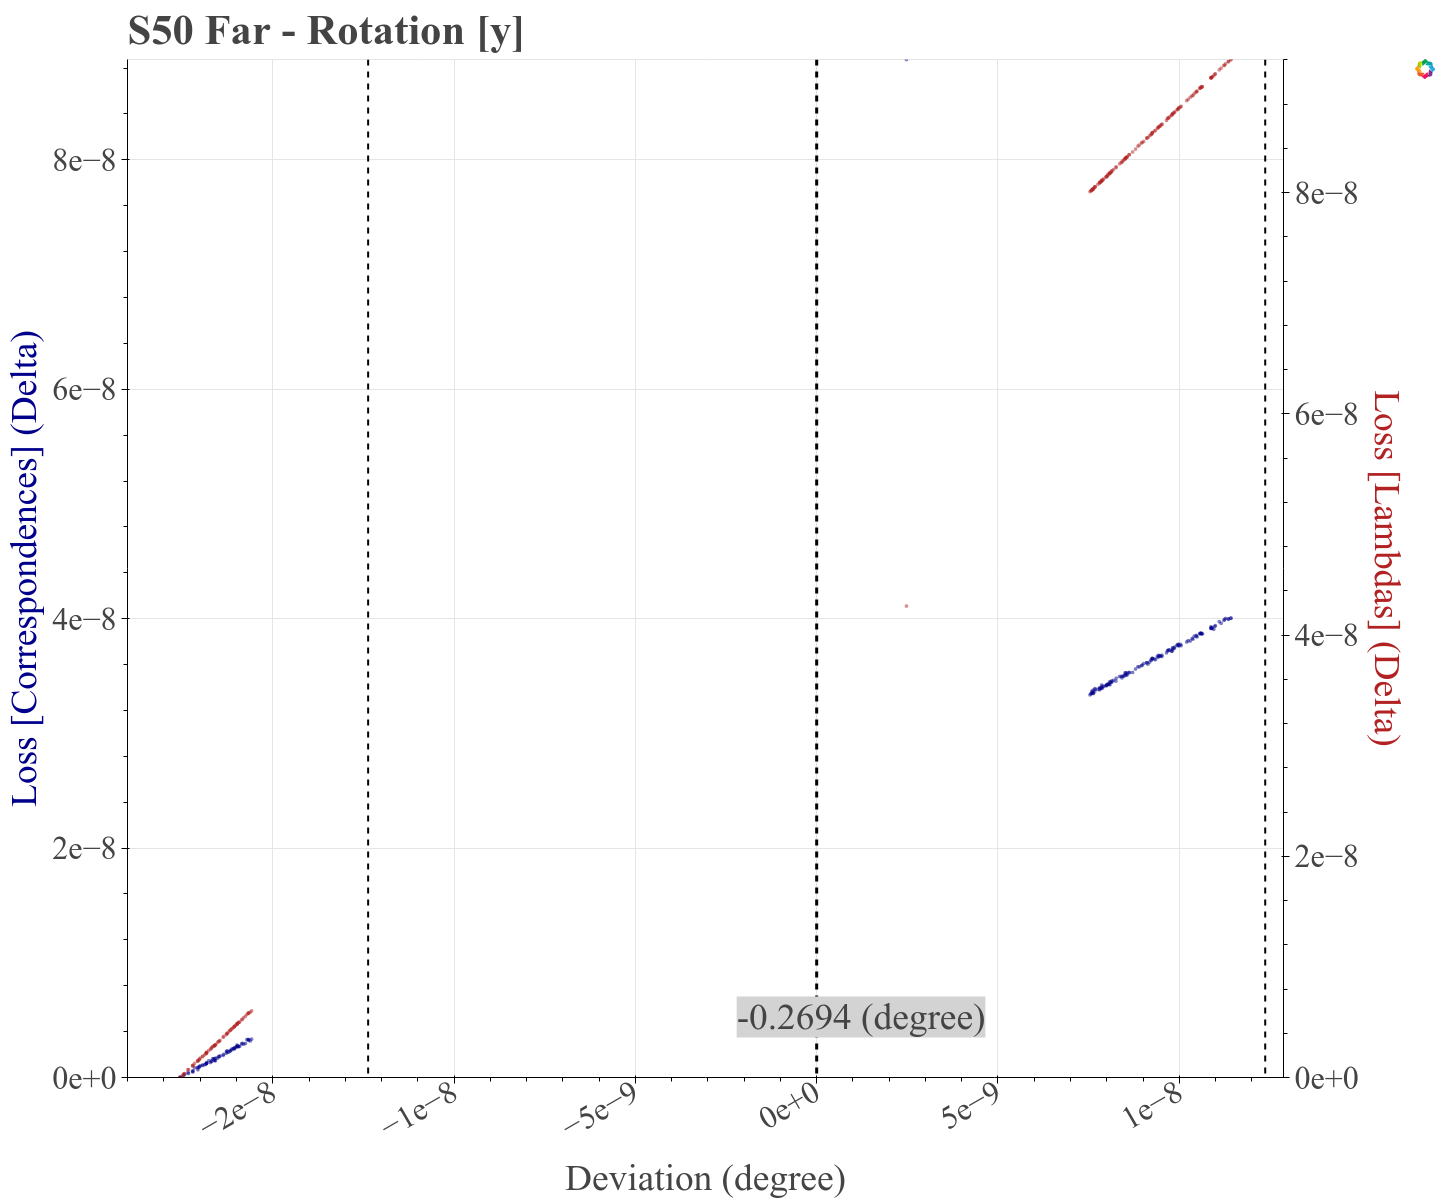
\includegraphics[width=0.45 \linewidth]{diagrams/calibration/s50_s_far/parameters.csv/Rotation[y]_vs_Loss[Correspondences]_vs_Loss[Lambdas]_cluster_All.png} \\
    
    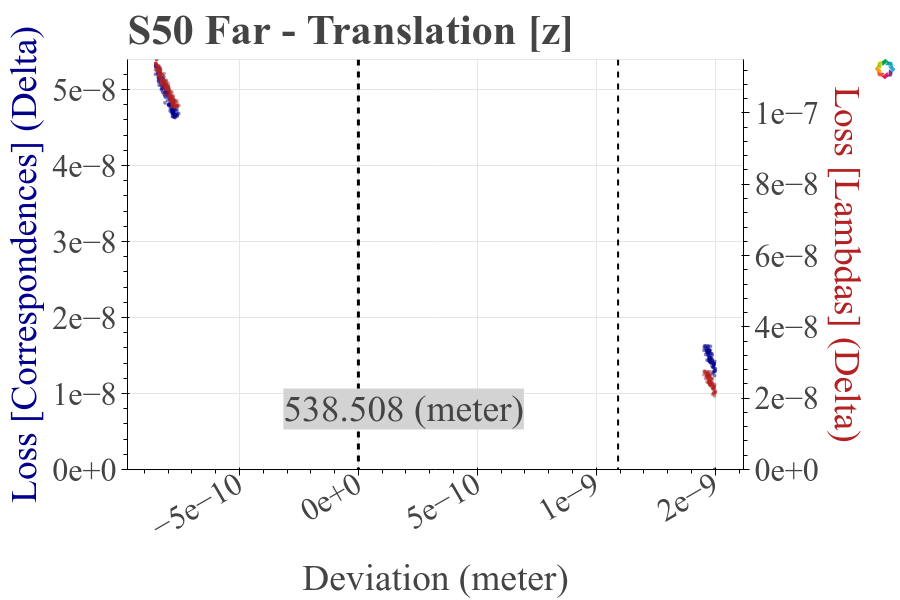
\includegraphics[width=0.45 \linewidth]{diagrams/calibration/s50_s_far/parameters.csv/Translation[z]_vs_Loss[Correspondences]_vs_Loss[Lambdas]_cluster_All.png} &
    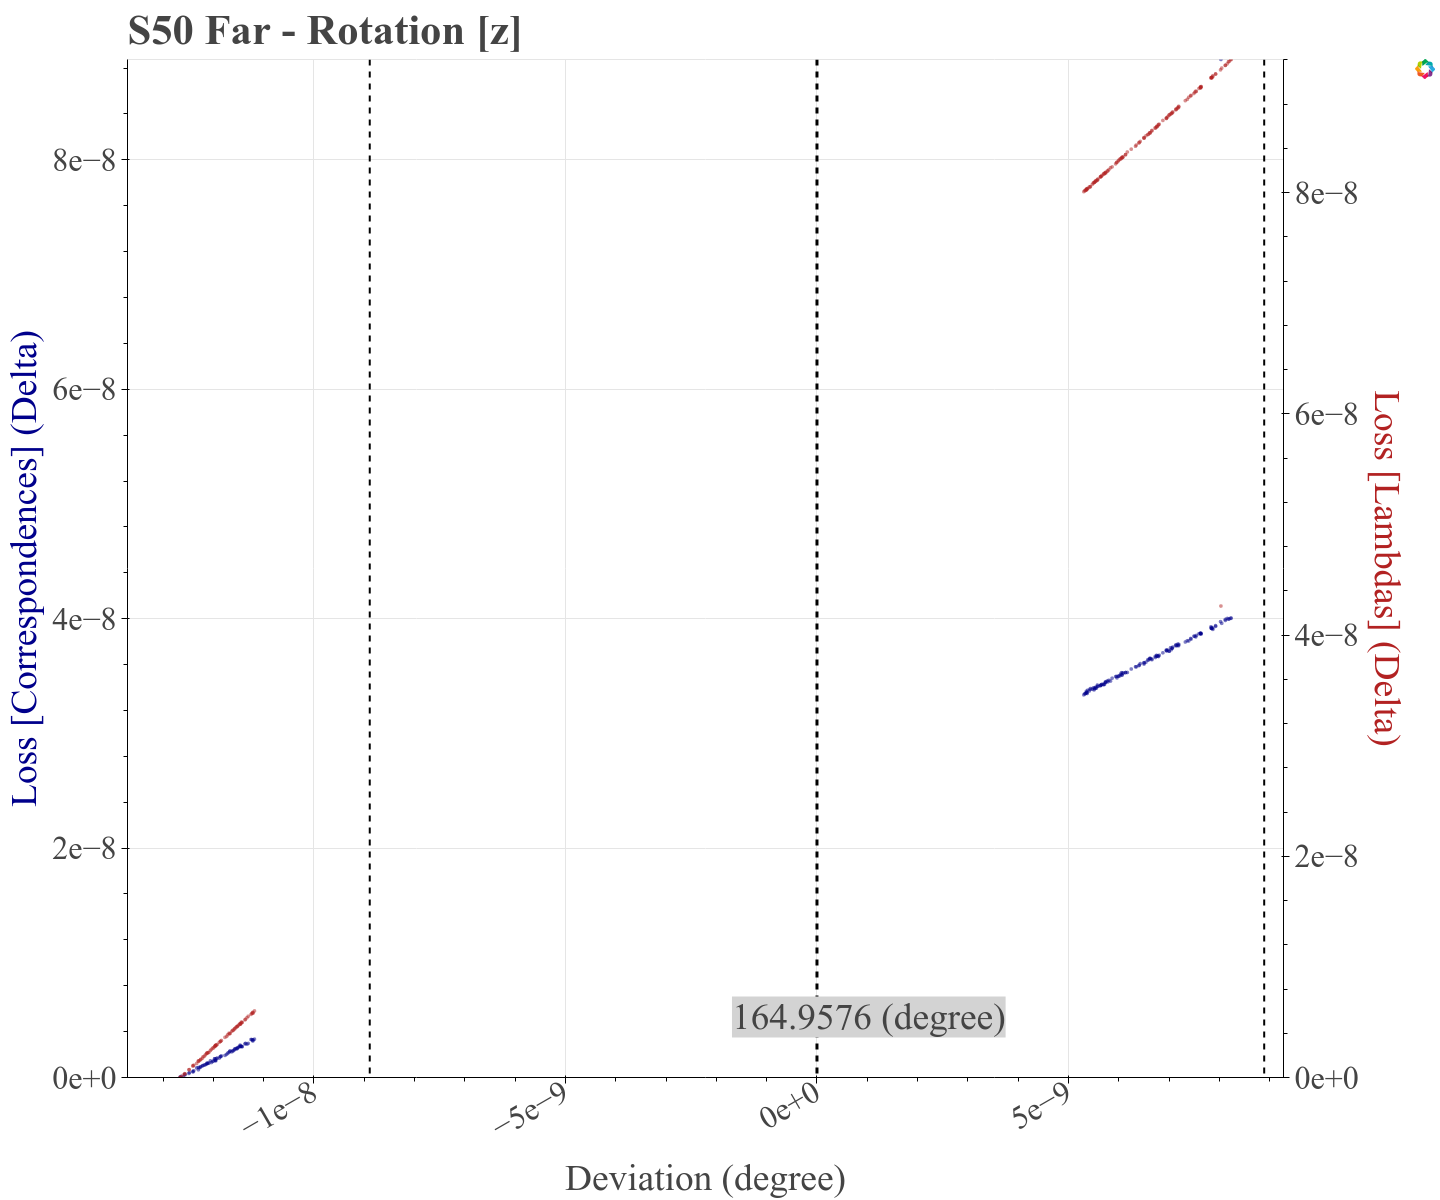
\includegraphics[width=0.45 \linewidth]{diagrams/calibration/s50_s_far/parameters.csv/Rotation[z]_vs_Loss[Correspondences]_vs_Loss[Lambdas]_cluster_All.png} \\

    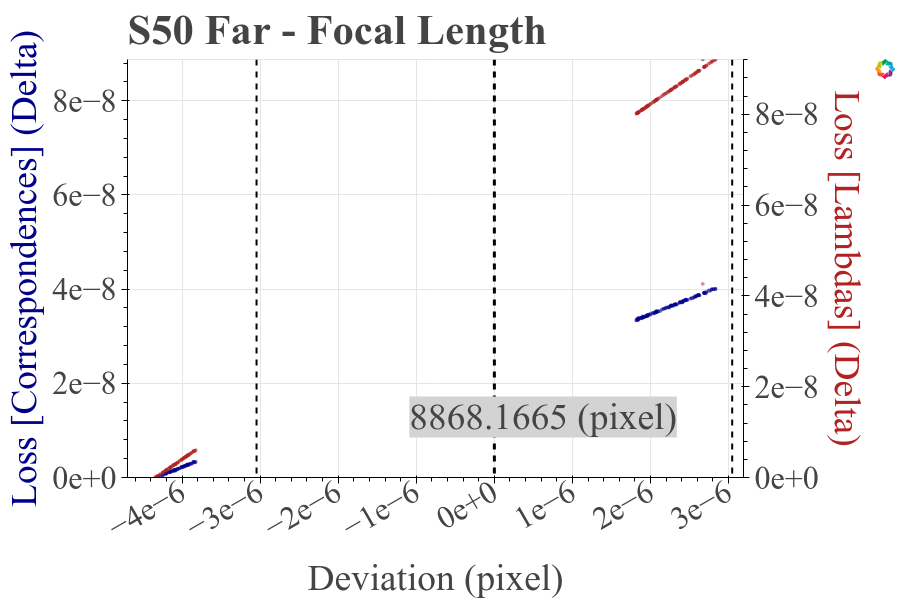
\includegraphics[width=0.45 \linewidth]{diagrams/calibration/s50_s_far/parameters.csv/FocalLength_vs_Loss[Correspondences]_vs_Loss[Lambdas]_cluster_All.png} &

  \end{tabular}
\caption{
  Left: The resulting translational parameters plotted against the remaining losses. 
  Right: The resulting rotational parameters plotted against the remaining losses.
  Bottom: The resulting focal length  plotted against the remaining losses.
    }
\label{fig:static_calibration_algorithmic_error_s50_s_far}
\end{figure*}

\begin{figure*}[!ht]
  \centering
  \begin{tabular}{cc}
    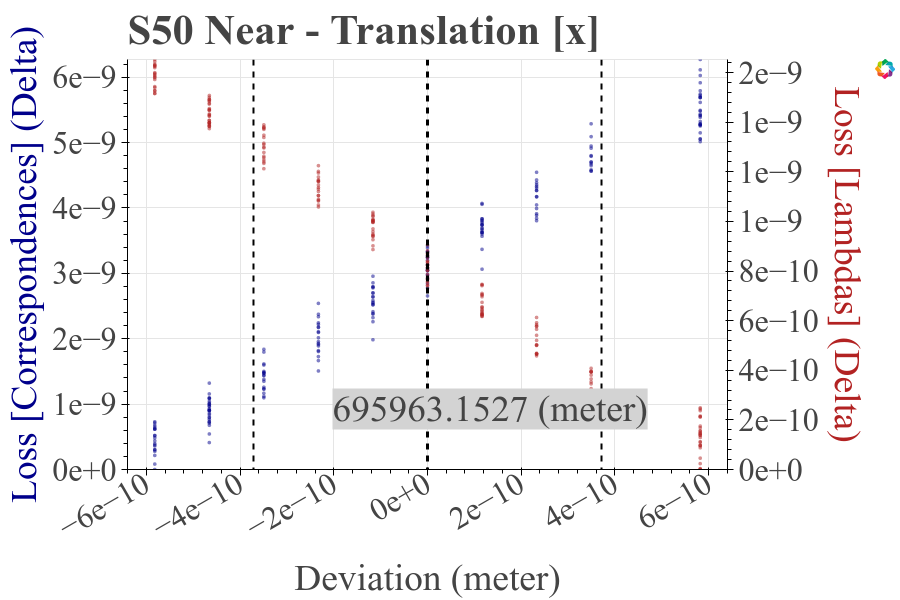
\includegraphics[width=0.45 \linewidth]{diagrams/calibration/s50_s_near/parameters.csv/Translation[x]_vs_Loss[Correspondences]_vs_Loss[Lambdas]_cluster_All.png} &
    \includegraphics[width=0.45 \linewidth]{diagrams/calibration/s50_s_near/parameters.csv/Rotation[x]_vs_Loss[Correspondences]_vs_Loss[Lambdas]_cluster_All.png} \\
    
    \includegraphics[width=0.45 \linewidth]{diagrams/calibration/s50_s_near/parameters.csv/Translation[y]_vs_Loss[Correspondences]_vs_Loss[Lambdas]_cluster_All.png} &
    \includegraphics[width=0.45 \linewidth]{diagrams/calibration/s50_s_near/parameters.csv/Rotation[y]_vs_Loss[Correspondences]_vs_Loss[Lambdas]_cluster_All.png} \\
    
    \includegraphics[width=0.45 \linewidth]{diagrams/calibration/s50_s_near/parameters.csv/Translation[z]_vs_Loss[Correspondences]_vs_Loss[Lambdas]_cluster_All.png} &
    \includegraphics[width=0.45 \linewidth]{diagrams/calibration/s50_s_near/parameters.csv/Rotation[z]_vs_Loss[Correspondences]_vs_Loss[Lambdas]_cluster_All.png} \\

    \includegraphics[width=0.45 \linewidth]{diagrams/calibration/s50_s_near/parameters.csv/FocalLength_vs_Loss[Correspondences]_vs_Loss[Lambdas]_cluster_All.png} &
\end{tabular}
\caption{
  Left: The resulting translational parameters plotted against the remaining losses. 
  Right: The resulting rotational parameters plotted against the remaining losses.
  Bottom: The resulting focal length  plotted against the remaining losses.
     }
\label{fig:static_calibration_algorithmic_error_s50_s_near}
\end{figure*}
